\subsection{Main}

To begin this iteration, we will start by implementing the base of the game. To start with, we will import PyGame, and define the display size and mode and tick rate. This is in \m{main.py}.
\vs

\begin{mpy}
#PyGame modules
import pygame
from pygame.locals import *
import sys
\end{mpy}

\vs
We will be running the game at 240 frames per second, which will be a lot higher than what most people will really be able to run the game at, but there is a good reason for this. With this high frame rate, we will get smooth gameplay regardless of the monitor's frame rate. This justifies it because it provides a similar experience for everyone playing the game, and will mean that the computer's hardware is taken full advantage of. We will be using frame-rate independent physics in order to ensure a fair game regardless of a person's device. Additionally, when we are training the AI, we will be disabling rendering, since it serves no purpose to use a rendering tool. This will allow for a substantial increase in performance and allow for very quick training.
\vs
\subsection{Game State Manager}

\vs
Now, we will create a game state manager. This will handle which state the game is currently in, and which state it will move to next. We will also pass global information, like timers, display size, refresh rate, etc, to this game state manager so that the other states, menus and the game loop itself can access this information.

\vs
\begin{mpy}
class GameStateManager:
  def __init__(self, current_state, SCREEN_DIMS, REFRESH_RATE):

    #Get the global game variables in a convenient way
    #Allows all states to easily access these values
    self.current_state = current_state
    self.SCREEN_DIMS = SCREEN_DIMS
    self.REFRESH_RATE = REFRESH_RATE

  #Returns the current state of the game
  def getState(self):
    return self.current_state

  #Set the next state of the game (ie. game loop -> game over)
  def setState(self, state):
    self.current_state = state
\end{mpy}

\vs

We can try and set and get states from the \m{GameStateManager} as follows.

\vs
\begin{mpy}
>>> gsm = GameStateManager('start', SCREEN_DIMS, REFRESH_RATE)
>>> gsm.get_state()
start
>>> gsm.set_state('next_state')
>>> gsm.get_state()
next_state
\end{mpy}
\vs
We assign the game state manager's attributes as the inputs we have defined. There will only be one instance of the game state manager, and therefore, this is going to allow us to access the game state manager within every state. However, in order to do that, we need to pass the instance of the manager into each of the states.


\vs

\subsection{\textcolor{blue}{Player}}

We need to define a player class, a menu class and a weapon class. This will form the basis of our game.
\vs

\begin{mpy}
class Player(pygame.sprite.Sprite):

  def __init__(self, spawn_point, initial_forward_vec, team, weapon):

    #Initialise the PyGame sprite
    pygame.sprite.Sprite.__init__(self)

    #Where the player will spawn every time they are killed
    self.spawn_point = spawn_point

    #The direction the player will face when they are respawned
    self.initial_forward_vec = initial_forward_vec

    #The maximum health that the player can have at any time
    self.max_health = 100

    #The current health of the player
    self.health = 100

    #The maximum magnitude of the velocity
    self.max_speed = 300

    #Which team the player is on, it will be an integer (0 or 1)
    #To check for a hit between two enemies
    #XOR the teams of the two players involved (0 means no hit, 1 means hit)
    self.team = team

    #The player's Weapon
    self.weapon = weapon

    #Current position of the players
    self.position = self.spawn_point

    #Current direction of the player
    self.forward_vec = self.initial_forward_vec

    #Radius of the circle representing the player
    self.radius = 75
\end{mpy}
\vs
The first, most obvious thing to implement is a way to move the player. This must be done using the inputs from the keyboard. We will set a maximum velocity, and use the keyboard inputs to find this value. However, we will do this in the game loop. For now, we will be implementing a move function, which will let us move the player on the map depending on the input. This is helpful, because this input could come from a human player, or an AI.
\vs

\begin{mpy}
  def move_player(self, directions, dt):
    #velocity = [Forward, Right] components
    velocity = [0, 0]

    #For loop avoids repeated code
    for i in (0, 2):
      if directions[i] == directions[i+1]:
        velocity[i//2] = 0
      else:
        velocity[i//2] = directions[i] - directions[i+1]

    #Velocity will have -1, 0, or 1 in each spot
    #If it is moving diagonally, x^2 + y^2 = 2
    #So we must divide the components by sqrt(2)
    if (velocity[0]**2 + velocity[1]**2 == 2):
      velocity = [i / 2**(1/2) for i in velocity]

    #We need to multiply by the max speed in order to get our final velocity
    velocity = [self.max_speed * i for i in velocity]

    #We will finally update the position of the player
    self.position = [self.position[i] + velocity[i]*dt for i in (0, 1)]


\end{mpy}
\vs

We can test this code as shown below. 

\begin{mpy}
>>> p = Player([4000, 4000], [0, -1], None, None)
>>> p.move([0, 0, 0, 0], 1)
>>> p.position
[4000, 4000]
>>> p.move([1, 1, 0, 0], 1)
>>> p.position
[4000, 4000]
>>> p.move([1, 0, 1, 0], 1)
>>> p.position
[4353.553390593273, 4353.553390593273]
\end{mpy}

\vs
This is what we have expected and so this function works as expected. The input to the function will be sanitised in the game loop, so there is no way for a user to enter invalid inputs. However, there is one thing we need to do. Primarily, we need to find a way to limit the player's movement between 0 and 8000. This can be done as follows.

\begin{mpy}
    #Update position of player
    updated_position = [self.position[i] + velocity[i]*dt for i in (0, 1)]

    #Check that the values are within (0, 0) and (8000, 8000)
    #(0, 0) is the top left of the map
    #(8000, 8000) is the bottom right

    for i in range(2):
        
      if updated_position[i] - self.radius <= 0:
        updated_position[i] = self.radius

      elif updated_position[i] + self.radius >= 8000:
        updated_position[i] = 8000 - self.radius

    self.position = updated_position
\end{mpy}

\vs

As mentioned in the design section, we want to only render the area around the player, and hence, we will define a \m{CameraPosition}. This will let us draw only things which are on the screen relative to the player. We can calculate the relative position of the players relative to this camera position, since we will also be using bots in the game. However, if the \m{Player} instance is for the user, then, it will just return the centre of the screen, because we want to keep the player at the centre of the screen.
\vs
\begin{mpy}
  #Will convert the world position of the character to a camera position for the player
  def convertToScreen(self, camera_position, object_position, SCREEN_DIMS):
    screenPosition = [object_position[i] - camera_position[i] + SCREEN_DIMS[i]//2 for i in (0, 1)]
    return screenPosition

\end{mpy}
\vs
We will also write a rendering function, in order to remove this from the game loop, which is helpful because different objects will be rendered differently, but letting all of them have their own render functions, will let us loop through all of the objects on the map and render them effectively.
\vs
\begin{mpy}
  #Renders the character to the display of the player
  def render(self, display, camera_position, directions, dt, SCREEN_DIMS):
    #Add code to not render if outside frame
    pygame.draw.circle(display, self.colour, self.convertToScreen(camera_position, self.position, SCREEN_DIMS), self.radius)
    for_pos = [self.position[i] + 100*self.forward_vec[i] for i in range(2)]
    pygame.draw.aaline(display, (100, 0, 0), self.convertToScreen(camera_position, self.position, SCREEN_DIMS), self.convertToScreen(camera_position, for_pos, SCREEN_DIMS))
    self.move_player(directions, self.forward_vec, dt)
\end{mpy}

The player is rendered as just a circle for now, maybe later to be replaced with something else. The \m{pygame.draw} methods are from the documentation, and we convert the position to the screen position so that the player remains stationary relative to the screen and everything else moves relative to them. This will ensure a more intuitive game experience.

\subsection{\textcolor{blue}{Database Handling}}

We will be using SQLite 3, since the project is small and likely to have only a few users. We are also not editing extremely frequently, only to create users, to login / register, or to update accounts after a game. Therefore, we can create a class to handle the management of the database, which we will call \m{DatabaseHandler}. We will define \m{SetupConnection()}, which will let the class instance connect to the database, and \m{CloseConnection()}, which will safely close the connection. This will ensure that we don't have issues in committing our changes to the database, and will ensure data safety.

\vs
\begin{mpy}
class DatabaseHandler:

  #Setup a cursor and connection in order to allow for queries and updates
  def SetupConnection(self):
    self.connection = sqlite3.connect("momentum_users.db")
    self.cursor = self.connection.cursor()

  #Close connection to prevent database corruption or multiple write attempts
  def CloseConnection(self):
    self.connection.close()
\end{mpy}
\vs
We will also define two more methods on our class, which are \m{CreateAccount()}, and \m{UpdateAccount()}, which are pretty self-explanatory. We want to be able to maintain referential integrity and atomicity, so for that reason only commit once all of the instructions that need to be commited have been passed to the cursor. This is important because it means that if there is an issue in one of the statements, then we don't break referential integrity across the database. There is no way to really check that these commands work, so we will just have to use them in the next commands ensure that they work there. There are no inputs from this, so we can't really "break" these functions anyway.

\vs
\begin{mpy}
  def CreateAccount(self, PlayerID, Email, Password):
    #Setup connection and cursor
    self.SetupConnection()

    #Insert data into each of the tables individually
    self.cursor.execute(f"INSERT INTO Player VALUES('{PlayerID}', '{Email}', '{Password}')")
    self.cursor.execute(f"INSERT INTO PlayerXP VALUES('{PlayerID}', 0)")
    self.cursor.execute(f"INSERT INTO MMR VALUES('{PlayerID}', 1000)")
    self.cursor.execute(f"INSERT INTO Matches VALUES('{PlayerID}', 0, 0)")

    #Commit and close connection
    self.connection.commit()
    self.CloseConnection()

  def UpdateAccount(self, PlayerID, PlayerXP, MMR, MatchWon):
    #Setup connection and cursor
    self.SetupConnection()

    #Update each statistic
    self.cursor.execute(f"UPDATE PlayerXP SET PlayerXP = PlayerXP + {PlayerXP} WHERE PlayerID = '{PlayerID}'")
    self.cursor.execute(f"UPDATE MMR SET MMR = {MMR} WHERE PlayerID = '{PlayerID}'")
    self.cursor.execute(f"UPDATE Matches SET MatchesPlayed = MatchesPlayed + 1, MatchesWon = MatchesWon + {MatchWon} WHERE PlayerID = '{PlayerID}'")

    #Commit and close connection
    self.connection.commit()
    self.CloseConnection()

\end{mpy}
\vs
In the \m{UpdateAccount()} method, we have simply taken the change in PlayerXP and whether the Match was won or not. This is helpful because it reduces the number of calls we need to make. This is because, we know that if we are calling this method, we have just completed another game, and so the number of matches played must increase by one, and whether the match was won or not is simply just a one or a zero. This means we don't need to find this information from the database using a query before inserting it back. This also reduces the chance of some error happening during this transition, and reduces the time taken.
\vs

We will now test these functions to make sure that they work and that we can succesfully link to the database. To ensure that this happens, we first need to create a database. This will follow the specification laid out in the design section. We will be using SQLite3 here, since it is a lightweight framework to use instead of a more concrete SQL package which would take a significant amount of work to setup.

\vs
We can test it as follows. We will use the functions to create and update an account, and then use another function to get this data back. We will now construct the function to get the user information. This will also be useful when constructing the leaderboard. We will first use \m{fstring} in order to format the strings in a concise and quick manner. This is shown as below.

\vs
\begin{mpy}
>>> PlayerID = "Ojas"
>>> f"SELECT * WHERE PlayerID = '{PlayerID}'"
"SELECT * WHERE PlayerID = 'Ojas'"
\end{mpy}

\vs
This is used as follows. For now, this will just return the data from one table, but we can expand it to give back the data from all of our tables. We can return the information as a dictionary which will make the data more processable and easier to work with.

\vs
\begin{mpy}
  def fetchUserInfo(self, PlayerID):
    self.SetupConnection()

    userInfo = {'PlayerID': PlayerID}

    result = self.cursor.execute(f"SELECT * FROM Player WHERE PlayerID = '{PlayerID}'")

    userInfo['email'] = result[1]
    userInfo['password'] = result[2]

    return userInfo
\end{mpy}

We will now insert the following data into our database using the \m{CreateAccount()} method. We will then use the method above to get more data back.

\begin{mpy}
>>> dbh = DatabaseHandler()
>>> DatabaseHandler.CreateAccount("ojas_tiwari", "tiwariojas@gmail.com", "HelloAgain")
>>> dbh.fetchUserInfo("ojas_tiwari")
{'PlayerID': 'ojas_tiwari', 'email': 'tiwariojas@gmail.com', 'password': 'HelloAgain'}
\end{mpy}

This proves that our connection works, and that we can create accounts and fetch some user information. We will add to the \m{fetchUserInfo()} method when we need more information on the player.
\vs


Finally, we also need to define an authentication query, which will return true or false, depending on whether the user has inputted the correct credentials for their account. We will return a list, with one element if they have submitted the correct credentials, simplying containing \m{[True]}. Otherwise, they will get an array with two elements, the first containing \m{False}, and the second element will be the reason for their query being rejected either \m{'invalid_id'} or \m{'invalid_password'}. These are fairly self-explanatory, and will be used to show the user why the could not login.
\vs
\begin{mpy}
  def AuthenticateAccount(self, PlayerID, Password):
    #Setup connection and cursor
    self.SetupConnection()

    #Query player database
    result = self.cursor.execute(f"SELECT Password FROM Player WHERE PlayerID = '{PlayerID}'").fetchone()

    #Nothing to commit here, just close
    self.CloseConnection()

    #Use of a guard clause instead of a double conditional
    if result == None:
      return [False, 'invalid_id']
    if Password == result[0]:
      return [True]
    return [False, 'invalid_password']
\end{mpy}
\vs
We have used a guard clause in order to decrease the amount of code written.

\subsection{\textcolor{blue}{Utilities}}

We need to be able to do many vector operations quickly without having to re-write the code consistently. This also allows us to more easily test all of these methods and ensure that they are working properly. We need to be certain that they are accurate and are providing reproducible results. To that extent, we will define a new class \m{Utility} which will handle all of these calls. A lot of these vector calculations are quite complicated so to that end they have been referenced from other resources and have been listed in this document. I have put this towards the start of the development section since, lots of other things rely on this, and it was essential to getting the rest of the code to work.

\vs
We begin by defining our class.
\begin{mpy}
class Utility:

  def __init__(self):
    #Nothing to do here so far
    pass

  def dot(self, a, b):
    return sum([i*j for i, j in zip(a, b)])
\end{mpy}

\vs
The first method we have implemented is the dot product. For geometric vectors this is defined as 
\begin{align*}
  \vec{a} \cdot \vec{b} &= \sum_i a_i b_i\\
\end{align*}
Where $a_i$ refers to the $i$-th element of $\vec{a}$. Then, in Python, we can use the \m{zip()} function in order to get a list of tuples of corresponding elements, as shown below.
\begin{mpy}
for i in zip([1, 2, 3], [4, 5, 6]):
  print(i)

>>> (1, 4)
  (2, 5)
  (3, 6)
\end{mpy}

\vs
Then, we want to multiply the numbers in each pair together. We can directly access the elements using $i, j$ instead of just $i$ in the for loop, and thus we can instantly multiply them. We then create a list of these which produces this output.

\begin{mpy}
dottedVals = []
for i, j in zip([1, 2, 3], [4, 5, 6])
  dottedVals.append(i * j)
print(dottedVals)

>>> [4, 10, 18]
\end{mpy}

\vs
Finally, we need to take the sum of all of these, which we can do using \m{sum()}. This finally gives us the following.

\begin{mpy}
sum(dottedValues)

>>> 32
\end{mpy}
However, we can condense this code slightly, by using list comprehension. We can rewrite \m{dottedVals} as follows, and can then just remove it all together.

\vs
\begin{mpy}
dotProdut = sum([i * j for i, j in zip(a, b)])
\end{mpy}

\vs
We can test this out using two dummy arrays. I also don't want to create instances of the \m{Utility} class as this will occupy even more memory.

\begin{mpy}
>>> a, b = [1, 2, 3], [4, 5, 6]
>>> Utility.dot(a, b)
TypeError: Utility.dot() missing 1 required positional argument: 'b'
\end{mpy}
\vs

In order to solve this, there are two approaches. Firstly, we could just create an instance of the \m{Utility} class, and then call the function. However, we do not want to do this because this would occupy a lot more memory.

\vs
The other alternative is to use the \m{@staticmethod} decorator and to remove \m{self} parameter from the function definition. The code then works as expected.

\begin{mpy}
>>> Utility.dot([1, 2, 3], [4, 5, 6])

32
\end{mpy}
Finally, I also considered using the library \m{NumPy} to do the dot product as it is already implemented. To decide which one to use, I decided to test it out by looking at how long it took to dot product lots of arrays. Since all of my vectors are 2D, they will only have 2 elements, and so that is what I used here.

\vs
\begin{mpy}
import numpy as np
import time
import random

time1 = time.time()

for i in range(10000):
  a = [random.random() for i in range(2)]
  b = [random.random() for i in range(2)]
  x = int(np.dot(a, b))
  
print("NumPy:", time.time()-time1)


class Utility:
  @staticmethod
  def dot(a, b):
    return sum([i*j for i, j in zip(a, b)])
    
time3 = time.time()

for i in range(10000):
  a = [random.random() for i in range(2)]
  b = [random.random() for i in range(2)]
  y = Utility.dot(a, b)
  
print("Raw Python:", (time.time() - time3))
\end{mpy}
\vs
Looking at the results, we see that the raw Python implementation is much faster than the \m{NumPy} implementation. This is likely due to the fact that \m{NumPy} needs to convert lists into \m{NumPy} arrays in order to be able to compute the dot product.

\begin{mpy}
NumPy: 0.3286013603210449
Raw Python: 0.17571258544921875
\end{mpy}
\vs
Therefore, I will use the Python implementation.

\vs
Additionally, we will construct addition and subtraction for vectors. Another possible consideration was to just use NumPy throughout the game, and I don't know why I didn't do this.... 

\begin{mpy}
  @staticmethod
  def vecSub(a, b):
    return [i-j for i, j in zip(a, b)]

  @staticmethod
  def vecAdd(a, b):
    return [i + j for i, j in zip(a, b)]
\end{mpy}
\vs

We can test these out as shown below.
\vs

\begin{mpy}
>>> Utility.vecSub([4, 5, 6], [1, 2, 3])
[3, 3, 3]
>>> Utility.vecAdd([1, 2, 3], [4, 5, 6])
[5, 7, 9]
\end{mpy}

\vs
Next, we will need to implement a collision between a ray and a circle. This is important as this will be used to detect when a weapon has fired a ray that has hit another player. We will be using the implementation from \href{https://codereview.stackexchange.com/questions/86421/line-segment-to-circle-collision-algorithm}{this StackExchange post}, which uses vectors in order to solve this problem. This is much more efficient than using Cartesian co-ordinates.

\vs
\begin{mpy}
  @staticmethod
  def lineCircleCollision(line, circle):
  
    #Notation from the StackExchange post
    q = circle[0]
    r = circle[1]
    p1 = line[0]
    v = Utility.vecSub(line[1], p1)

    a = Utility.dot(v, v)
    b = 2 * Utility.dot(v, Utility.vecSub(p1, q))
    c = Utility.dot(p1, p1) + Utility.dot(q, q) - 2 * Utility.dot(p1, q) - r**2

    discriminant = b**2 - 4 * a * c

    if discriminant < 0:
      return [False, None]

    sqrt_disc = sqrt(discriminant)
    
    t1 = (-b + sqrt_disc) / (2 * a)
    t2 = (-b - sqrt_disc) / (2 * a)

    if not (0 <= t1 <= 1 or 0 <= t2 <= 1):
      return [False, None]
    
    t = min(t1, t2)
    return [True, t]
\end{mpy}

\vs
In this implementation, we do not provide a direction vector, rather we provide two constraint points. This solution is much more optimal, since it means we do not also need to provide a range parameter. We simply want to find the closest collision to the source, and this will provide it if a collision is found. The $t$-value must be between $0$ and $1$ where $0$ would mean that the source is right next to the circle we are checking for a collision with, and $1$ means that the second constraint point lies on the circle. We can test this code out as follows.

\vs

We will first check the two standard cases; one where the collision does occur and one where it doesn't.

\begin{mpy}
>>> line = [[0, 0], [10, 5]]
>>> circle = [[2, 3], 2]
>>> Utility.lineCircleCollision(line, circle)
[True, 0.2]
\end{mpy}

\vs
We can check manually, or using plotting software that this does indeed work. We will now check when there should not be a collision.

\vs
\begin{mpy}
>>> line = [[2, 3], [-5, -6]]
>>> circle = [[5, 10] , 2]
>>> Utility.lineCircleCollision(line, circle)
[False, None]
\end{mpy}
\vs
This is as expected. Next, we will test when the second constraint is just on the circle.

\vs
\begin{mpy}
>>> line = [[0, 0], [5, 0]]
>>> circle = [[6, 0], 1]
>>> Utility.lineCircleCollision(line, circle)
[True, 1.0]
\end{mpy}
Again, this is the result we expected.

\vs
We will test the case where the first constraint is inside of the object, but not the second.
\begin{mpy}
>>> line = [[0, 0], [5, 10]]
>>> circle = [[2, 0], 2]
>>> Utility.lineCircleCollision(line, circle)
[True, 0.0]
\end{mpy}
\vs
Finally, despite this case never arising in an actual game, we will test the case where both constraints are inside of the circle.
\begin{mpy}
>>> line = [[0, 0], [0, 1]]
>>> circle = [[0, 0], 3]
>>> Utility.lineCircleCollision(line, circle)
[False, None]
\end{mpy}
Again, the desired result! So, we can conclude that the function works as expected.
%https://www.jeffreythompson.org/collision-detection/line-rect.php

\vs
We will now implement the line-line collision method we which described thoroughly in the design section. We will be using NumPy to do the solving of the simultaneous equations. We first need to check that the equations are linearly independent. We can do this using the determinant of the matrix. We will first be extracting all of the elements we need to make the rest of the code easier to read.

\begin{mpy}
  @staticmethod
    def lineLineCollision(line1, line2):
      #We have both lines in vector form
      #line 1 -> [x_1, y_1], [x_2, y_2]
      #line 2 -> [x_3, y_3], [x_4, y_4]
      x_1, y_1 = line1[0]
      x_2, y_2 = line1[1]
      x_3, y_3 = line2[0]
      x_4, y_4 = line2[1]
\end{mpy}

After this we can compute the determinant and if it is not 0, we can find the solutions.
\begin{mpy}
    #Find the determinant
    determinant = np.linalg.det(matrix)
    if determinant == 0:
      return [False, None]
          
    else:
      result = np.linalg.solve(matrix, resultVec)
          
      #Check that the result is between the constraint points
      if 0 <= result[0] <= 1 and 0 <= result[1] <= 1:
        return [True, result]
      return [False, None]
\end{mpy}

We can also edit this code to make it more readable by using a guard clause. Since we are returning if the determinant is 0, no other code after it will return if this condition is meant. Therefore, we can see that we don't need the \m{else} statement at all, and can instead dedent the code block there.

\begin{mpy}
    #det = 0 -> Can't be solved
    if determinant == 0:
      return [False, None]

    #Solve system
    result = np.linalg.solve(matrix, resultVec)

    #Check that the result is between the constraint points
    if 0 <= result[0] <= 1 and 0 <= result[1] <= 1:
      return [True, result]
    
    #Solution is not in bounds
    return [False, None]
\end{mpy}

\vs
We also want to be able to test this code and make sure that is efficient, since we are casting to a NumPy array this likely to not be very efficient. We are primarily interested in how iterations we can do in one second, since this will be very helpful during the training, and we want to make sure that the environment is easy to sample with.

\begin{mpy}
start = time.time()
for i in range(70000):
  line1 = [[random.uniform(0, 8000), random.uniform(0, 8000)], [random.uniform(0, 8000), random.uniform(0, 8000)]]
  line2 = [[random.uniform(0, 8000), random.uniform(0, 8000)], [random.uniform(0, 8000), random.uniform(0, 8000)]]
  x = Utility.lineLineCollision(line1, line2)
end = time.time()
print(end - start)

>>> 1.0048434734344482
\end{mpy}

This quite significant which means that we can do a lot of timesteps in one second, which will increase our overall training speed.

\vs

The next thing we will be implementing is the line-rectangle collision. We can decompose each rectangle into 4 lines between adjacent corners. Therefore, we need to create a method to get the corners of a rectangle. Therefore, we will create a new method in the \m{Block} class to get the corners.

\vs
\begin{mpy}
  def getCorners(self):
    #TL, BL, BR, TR
    corners = []

    for i in range(-1, 2, 2):
      for j in range(-1, 2, 2):
        corners.append(U.vecAdd(self.centre, [i * self.length1/2, i * j * self.length2/2]))

    return corners
\end{mpy}

\vs
The code is a bit dense, but we can prove that this code will work and then test it. We want to get the corners in an anti-clockwise order because this will give us the lines that we since the lines must be on the edges of the rectangle. We firstly create an array to store the co-ordinates of the corners in. Next, we create two for loops. The outer loop will take two values only, $-1$ and $+1$. This will show the direction of the horizontal movement from the centre. In the inner loop, we can either move upwards by half of the height of the rectangle, or we can move down by the same amount. This produces all 4 corners. If we just print $i$ and $ij$, we can see that the output is as follows.

\begin{mpy}
>>> for i in range(-1, 2, 2):
  for j in range(-1, 2, 2):
    print(i, i*j)

-1 1
-1 -1
1 -1
1 1
\end{mpy}
\vs

This can be plotted on the $x$ and $y$ axes, which is going anti-clockwise, and we are only changing one element of the co-ordinate at a time which means that we will only be putting adjacent vertices next to each other.

\vs
We can now test the code with some sample values.

\begin{mpy}
b = Block([1, 2], 10, 20, 'red', [1600, 900], [800, 450])
corners = b.getCorners()
print(corners)

>>> [[-4.0, 12.0], [-4.0, -8.0], [6.0, -8.0], [6.0, 12.0]]
\end{mpy}

This is what we would have expected to see. Now, that we have this, we want to find the edges of the rectangle. With this, we can generate the edges present.

\vs
\begin{mpy}
  @staticmethod
  def lineRectCollision(line, block):

    #Get the corners
    corners = block.getCorners()
    
    #Decompose the rectangle into 4 lines: TL -> TR, TR -> BR, BR -> BL, BL -> TL
    lines = [[corners[i], corners[i+1]] for i in range(-1, 3) ]
\end{mpy}

\vs
The second line is list comprehension which gives pairs of corners, and since we have arranged them to be adjacent to each other, the lines formed are all on the boundary of the rectangle. We only need the pairs of constraint points since that is what we are using for the line collision method.

\vs
The next thing we need, is to find the collision which is the closest to the first constraint point which is what our program returns.
\vs

\begin{mpy}
    #We only care about how far along the main line the collision is
    t_val = 3
    for edge in lines:
      isHit, lambda_mu = Utility.lineLineCollision(line, edge)
      if isHit:
        if lambda_mu[0] < t_val:
          t_val = lambda_mu[0]
\end{mpy}

\vs
We set \m{t_val} to be $3$ since the result of the collision must be between 0 and 1, and so this will be well outside of the range anyway. This also means that we can check if we ever updated the minimum collision distance.

\vs
\begin{mpy}
    if t_val == 3:
      return [False, None]
    return [True, t_val]
\end{mpy}

\vs
We can also return whether we have detected a collision or not, and if we have, then what that distance is. We will be testing a boundary case, where the line clips one of the edges of a rectangle, but should still return a hit.

\begin{mpy}
b = Block([0, 0], 10, 20, 'red', [1600, 900], [800, 450])
line = [[0, 20], [10, 0]]
result = U.lineRectCollision(line, b)
print(result)

>>> [True, 0.5]
\end{mpy}

\vs
We also need to define the method for converting a world position to a screen position which will let us actually render things, since the player's viewpoint moves as the player moves. We can do this as detailed in the Design section.

\begin{mpy}
  #Will convert the world position of the character to a camera position for the player
  @staticmethod
  def convertToScreen(camera_position, object_position, SCREEN_DIMS):
    screenPosition = [object_position[i] - camera_position[i] + SCREEN_DIMS[i]//2 for i in (0, 1)]
    return screenPosition
\end{mpy}

\vs
We have used list comprehension to compress our statements, since this is more efficient than using a for loop (from \cite{listcomp}), since they do not have an overhead in producing a for loop, and therefore, we have used this throughout the project. This means that we can now easily and efficiently call all of these functions and due to the stateless nature of the \m{Utility} class we don't need to worry about creating and deleting many instances, and this is also more efficient to do in Python, which has been a concern throughout the project, since we will be removing the render functions and will be using the game loop to do the training of the game. Therefore, every aspect of the game must be optimised to a reasonable extent in order to allow for more samples in a given period of time. As a result of this we will be removing the \m{convertToScreen} method from the \m{Player} class since it is no longer needed since we have already globalised its implementation to the \m{Utility} class.

Another method that we should implement since this is very commonly used is the scalar multiple of a vector. For this, we need two inputs, one is a vector and another is a scalar by which we need to multiply the vector by. This is done by list comprehension again.

\begin{mpy}
  @staticmethod
  def mult(vec, scalar):
    return [i * scalar for i in vec]
\end{mpy}

We simply take each element of the vector and then multiply it by the vector we took in. We can test it as follows.

\begin{mpy}
>>> Utility.mult([1, 2], 2)
[2, 4]
\end{mpy}

Additionally, we need to be able to rotate vectors, specifically to create spread in the weapon's fire, such as for the shotgun. We can do this as fllows. We consider the matrix ($\hat{A}$) for a 2D rotation which is written as follows.

\begin{align*}
  \hat{A}(\theta) &= \begin{bmatrix} \cos \theta & - \sin \theta \\ \sin \theta & \cos \theta \end{bmatrix}\\
\end{align*}

We can do a simple matrix-vector product as follows.
\begin{align*}
  \vec{r} &= \begin{bmatrix} x \\ y \end{bmatrix}\\
  \vec{r}' = \hat{A}\vec{r} &= \begin{bmatrix} x \cos \theta - y \sin \theta \\ x \sin \theta + y \cos \theta \end{bmatrix}\\
\end{align*}

This can then be converted into code as follows.

\begin{mpy}
  @staticmethod
  def rotateVector(vec, angle):
    #https://matthew-brett.github.io/teaching/rotation_2d.html
    rotatedVec = [0, 0]
    rotatedVec[0] = vec[0] * cos(angle) - vec[1] * sin(angle)
    rotatedVec[1] = vec[0] * sin(angle) + vec[1] * cos(angle)

    return rotatedVec
\end{mpy}

The \m{sin()} and \m{cos()} functions are from the \m{math} library which was imported at the start of the file. We can test this function as follows.

\begin{mpy}
>>> Utility.rotateVector([1, 0], math.pi/4)
[0.7071067811865476, 0.7071067811865476]
>>> 2**-0.5
0.7071067811865476
\end{mpy}

This means that we have rotated the vector anti-clockwise by an angle of \ang{45} or $\frac{pi}{4}$ radians. Furthermore, we can test this for other angles as well like \ang{90}.

\begin{mpy}
>>> Utility.rotateVector([1, 0], math.pi/2)
[6.123233995736766e-17, 1.0]
\end{mpy}

This is not exactly right, but it is close enough to what we need since we expected 1.0 in the $y$-ordinate, and the $x$-ordinate is so incredibly small that we would not be able to process such as a change anyway.


\subsection{\textcolor{blue}{Weapon}}
We will give each player a weapon, of a specific class, which will have specified statistics. In order to do this, we can create a parent class \m{Weapon} and derive other weapons from it. There are a few specific attributes that we need to have for the parent class. 
\vs
\begin{mpy}
class Weapon:
  #We need a way to move the weapon alongside the Weapon
  #Some way to attach the two together
  #TODO
  def __init__(self):
    self.ammo = 30
    self.reloadTime = 2.0
    self.damagePerHit = 5
    self.range = 1000
    self.std_dev = 0.25
    self.cooldown = 0.2
    self.raysPerShot = 1
    self.cooldown = 0.25
    self.spread = 1
\end{mpy}

We will now justify each attribute. The ammo is the largest amount of ammunition that the weapon can fire before needing to reload. This is important since otherwise a player could just hold down the fire button without needing to be aiming correctly. The reload time is the amount of time taken from emptying the weapon's "cartridge" to refilling it so that they player can fire the weapon again.

\vs
The damage per hit is self-explanatory, but every time a ray from that weapon hits a player, this is the amount of damage that is dealt. The range is the maximum distance that the ray can extend, and is used to find the end point of the ray that we will be using for the ray collision detection.

\vs
The standard deviation is used for the normal distribution to find how spread out the rays will be from the direction vector. We will be firing rays from the player, and then find an angle to rotate this vector by to find the ray's direction. We can do this as follows.

\begin{mpy}
>>> std_dev = 0.25
>>> np.random.normal(loc = 0, scale=std_dev, size=None)
0.3018635745361101
>>> np.random.normal(loc = 0, scale=std_dev, size=None)
-0.12774112426206038
>>> np.random.normal(loc=0, scale=0.25, size=None)
0.043154759156613466
\end{mpy}
\vs
This will let us create derived classes from this and then assign them each different values for these attributes. Alongside this, we can define a fire function, which will let us project a ray from the weapon's position and direction, and hand it over to the game loop to identify any collisions. Importantly, the ray is defined $\mathbf{r} + t \mathbf{d}$, where $\mathbf{r}$ is the position of the player, and $\mathbf{d}$ is the direction.
\vs

Therefore, our player will need to pass the position and direction from the \m{Player} class. This will then return a tuple of vectors which we then pass to the game loop.
\vs

We will take firing as being a Boolean, either 0 or 1. This will be whether we are currently firing the weapon or not, and will be taken from a mouse input. Furthermore, we will take the direction that the mouse is pointing in to be the direction of the player. $t$ must greater than 0, because this will allow us to trace the ray as it progress forward from the player, since it wouldn't make sense for it to move behind the player.
\vs

We also need to create attributes for the number of rays per shot as well as the angle of the rays as they spread out. For example, for a sniper, there is only ray produced and it doesn't deviate from the direction vector. To add this randomness, we can generate a random angle between 0 and the maximum limit according to a normal distribution or a uniform distribution, and then rotate the direction vector around each time. This will return an array of rays, which can then be passed on. Hence, for all fire functions, we will be returning an array which is iterated over. We also add a spread factor which is a boolean and will tell the \m{fire()} method whether to include a spread or not.
\vs


The rays will be randomly spread out. We can do this as follows.
\begin{mpy}
  #We will attach the damage to this as well
  def fire(self, position, direction):
    rays = []
    magnitude_squared = U.dot(direction, direction)
    unit_dir = U.mult(direction, 1 / sqrt(magnitude_squared))

    for i in range(self.raysPerShot):

      #Sample deviation using the normal distribution
      if self.spread == 1:
        angleDeviation = random.normal(loc = 0, scale=self.std_dev, size=None)
        rotated_dir = U.rotateVector(unit_dir, angleDeviation)
      else: 
        rotated_dir = unit_dir

      #Add unit_dir rotation here using matrices
      final_extent = U.vecAdd(position, U.mult(rotated_dir, self.range))
      rays.append([position, final_extent, self.damage])

    return rays
\end{mpy}
\vs
We will now explain each bit of this code. We first create an array of rays, since there will be weapons which produces multiple rays. We also have the direction vector of the player, but this is not necessarily normalised, so for that reason, we will be normalising it first using the dot product and the scalar multiple of 1 over the magnitude. This is essential, since if the direction vector is not normalised the length of the ray will be longer than the actual ray which should occur. We then create a for loop for the number of rays that we want to produce, and then append these rays into the array.

\vs
We can produce these rays by first generating the angle that we want the ray to be deflected by, and then, rotating the vector by the amount that we want. The next step is to find the final position of the ray, which we can do with \m{U.vecAdd()} with the player position and the rotated direction vector.

\vs
We will create multiple weapons to create interactivity as mentioned before, and we can do this simply by editing the \m{__init__(self)} for each class as follows.

\begin{mpy}
#Automatic weapon, good at mid range
class AssaultRifle(Weapon):
  def __init__(self):
    pass

#Long range, with a very high damage per hit, but slow reloads
class SniperRifle(Weapon):
  def __init__(self):
    self.ammo = 5
    self.reloadTime = 5.0
    self.damagePerHit = 100
    self.range = 4000
    self.std_dev = 1e-2
    self.cooldown = 2.0
    self.raysPerShot = 1
    self.cooldown = 2.0
    self.spread = 0

#A very short range weapon
class Shotgun(Weapon):
  def __init__(self):
    self.ammo = 6
    self.reloadTime = 3.0
    self.damagerPerHit = 35
    self.range = 500
    self.std_dev = pi/6
    self.raysPerShot = 10
    self.cooldown = 0.75
    self.spread = 1
\end{mpy}

\subsection{\textcolor{blue}{Block}}

We need to implement the \m{Block} class in order to add more interactivity with the game.

\begin{mpy}
import pygame
from pygame.locals import *
from utils import Utility as U
\end{mpy}

We can now write the constructor for the class. We can define a rectangle with three principle parameters. We need the two side lengths of the rectangle and the centre position of the rectangle. We can write this as follows.

\begin{mpy}
class Block(pygame.sprite.Sprite):

#Length1 is in the x direction
#Length2 is in the y direction
def __init__(self, centre, length1, length2, colour, SCREEN_DIMS, camera_position):

  pygame.sprite.Sprite.__init__(self)

  self.centre = centre
  self.length1 = length1
  self.length2 = length2
  self.colour = colour

  self.initial_screenPosition = U.convertToScreen(camera_position, self.centre, SCREEN_DIMS)
  self.rect = pygame.Rect(self.initial_screenPosition[0], self.initial_screenPosition[1], self.length1, self.length2)
\end{mpy}

We will now examine each aspect of the code to ensure that it is valid. As mentioned before, to define the geometry of the rectangle we needed a few principle values, which we now have. We also need to define a colour, since this is what we will be using to render. We can now define the render function as follows.

\begin{mpy}
  def render(self):
    self.rect.center = U.convertToScreen(camera_position, self.centre, SCREEN_DIMS)
    pygame.draw.rect(display, self.colour, self.rect)
\end{mpy}

\subsection{\textcolor{red}{Game Class}}
Now, we will implement the game class. This will control the main running of the game, and will contain all of the global variables. We will call an instance of this class from the \m{main.py} file, and we will run all of our other game states from this class.
\vs

We will begin by creating \m{game.py}, and importing our modules into it.
\vs
\begin{mpy}
#PyGame modules
import pygame
from pygame.locals import *
import sys

#Menu, Player, Weapon classes
from menu import *
from player import Player
from weapon import Weapon
\end{mpy}
\vs
Next, we will create our \m{Game} class.
\vs
\begin{mpy}
class Game:

  #Initialise the game class
  def __init__(self, WIDTH, HEIGHT, REFRESH_RATE):

    #Initialise PyGame and the screen
    pygame.init()
    self.screen = pygame.display.set_mode((WIDTH, HEIGHT))
    pygame.display.set_caption("Momentum")
    pygame.display.set_icon(pygame.image.load('assets/momentum_icon.png'))
\end{mpy}
\vs
This first block of code will start PyGame for us, and let us then use its functionality. Additionally, we will create the screen on top of which we are drawing, and then set it's caption, which is the name of our game, Momentum. We will also load an icon which will go in the top left of the screen and will show the game's icon.
\vs


After that, we create the game clock, which is essential to running the game, and controlling the frame rate and physics.
\vs
\begin{mpy}
    #Create the game clock
    self.clock = pygame.time.Clock()
    self.dt = 0
\end{mpy}
\vs
We will now define some global variables which will tell us the height, width and refresh rate of the screen, which is passed onto all of the other states should they need it at any point. This is justified, because it allows for a much more reliable way of communicating this information to the states, and it will prevent us from hard coding it into the game, which would cause compatibility issues, although this is unlikely. It will let us also experiment with different values for these variables very quickly, making prototyping and testing with users easier.
\vs
\begin{mpy}
    #Global settings
    self.WIDTH = WIDTH
    self.HEIGHT = HEIGHT
    self.REFRESH_RATE = REFRESH_RATE
\end{mpy}
\vs
Next, we will create instances of all of our different states and the \m{GameStateManager} instance, and assign it to the game, so that it can handle them appropriately. The manager uses short strings to get and set the states, and so we will now define a dictionary to translate between strings and classes. This is a reasonable choice for this purpose, since arrays and linked lists would be less efficient. 
\vs
\begin{mpy}
    #Game State Manager and Game States
    self.gameStateManager = GameStateManager('game_loop', [self.WIDTH, self.HEIGHT], self.REFRESH_RATE)
    self.start = Start(self.screen, self.gameStateManager)
    self.options = Options(self.screen, self.gameStateManager)
    self.login = Login(self.screen, self.gameStateManager)
    self.register = Register(self.screen, self.gameStateManager)
    self.createGame = CreateGame(self.screen, self.gameStateManager)
    self.setTimer = SetTimer(self.screen, self.gameStateManager)
    self.gameLoop = GameLoop(self.screen, self.gameStateManager)
    self.gameOver = GameOver(self.screen, self.gameStateManager)
\end{mpy}
\vs
As mentioned before, we will need to define our dictionary to translate to game states from a string.
\vs
\begin{mpy}
    #Game States so that we can convert strings into instances
    self.states = {'start': self.start,
          'options': self.options,
          'login': self.login,
          'register': self.register,
          'create_game': self.createGame,
          'set_timer': self.setTimer,
          'game_loop': self.gameLoop,
          'game_over': self.gameOver
    }
\end{mpy}

\vs
Additionally, every time a state is run, it will return some type of return value. This is because it needs to be able to communicate with other states. These types may be different, but we will initialise it, since the main game loop will in fact be passing the previous return value in to the next game state. However, since the variable wouldn't exist, it would throw an error, and so we initialise it to prevent that, even though it is not required.
\vs
\begin{mpy}
    #A return value that we will pass into each new game state
    #Will contain things like, user info, score, etc
    self.returnValues = []
\end{mpy}


Now, we will define the main loop which will be running our game. This will contain a \m{while} loop, since we do not know how long the player will be playing for, and therefore, there is no other alternative. 


\begin{mpy}
  #Runs the main game
  def run(self):

    #Main Application Loop
    while True:

      #Get all events
      events = pygame.event.get()

      #Get all key presses
      keys = pygame.key.get_pressed()

      #Check if user wants to quit
      for event in events:
        if event.type == pygame.QUIT:
          pygame.quit()
          sys.exit()

      #Use flags to identify the return values, ie: returnValues[0] = 'score'
      #Maybe consider input Values into the run function?
      self.returnValues = self.states[self.gameStateManager.get_state()].run(self.returnValues)

      #Update the display
      pygame.display.update()

      #Update the clock
      dt = self.clock.tick(self.REFRESH_RATE)/1000
\end{mpy}
\vs
This will let us accept the new return values from the game, and input the previous ones into the new state and run it. Each state will have it's own \m{while} loop which will allow it to run some code. 

\vs
Now that we have the fundamental layout of the game completed, we will update our \m{main.py} file to allow it to use all of the capabilities that we have now implemented. This is as follows.
\vs
\begin{mpy}
import pygame
from pygame.locals import *
import sys

#Import Game class
from game import Game

#Global settings
REFRESH_RATE = 240
HEIGHT = 1080
WIDTH = 1920

#Game class
g = Game(WIDTH, HEIGHT, REFRESH_RATE)

#Run the game
g.run()
\end{mpy}

This will import the \m{Game} class and will create an instance, and run the game. What this means is that we can now draw things on the screen and run the code as one complete system. This simplifies iterative testing a lot. For now, we will take two menus, and just draw them as being different colours and switch between them to prove that the main game works.

\vs
We will create two classes, \m{MenuA} and \m{MenuB}. \m{MenuA} will be shaded in blue and \m{MenuB} will be in red. This will help to distinguish between the two. If we are in \m{MenuA} and we press the down key, we will move to \m{MenuB}, and if we are in \m{MenuB} and we press the up key, we want to move to \m{MenuA}. This can be done as follows.

\vs
We will now demonstrate that this works, by putting some text on each menu object, and then passing commands to each of these to update the state. This works as follows. We will create a main \m{Menu} class, since most of the methods and functions will be similar between each menu class. This will make our job much easier and prevent us from writing the same code over and over again. This will make use of inheritance, with each menu being the child of the main menu class, and using \m{specificMethod} to create a function which will run specifically in the loop for each menu class. We can feed the inputs and events from the main loop into the specific method. This will drastically reduce the amount of code we need, and since most menus are relatively similar, this will not limit us in any way.




\vs
The \m{Menu} class has a constructor as follows.
\begin{mpy}
class Menu:
  def __init__(self, display, gameStateManager, bgColor):

    #Set the display on which we are rendering
    self.display = display
    
    #Set the gsm
    self.gameStateManager = gameStateManager

    #Set screen dims
    self.SCREEN_DIMS = gameStateManager.SCREEN_DIMS

    #Set bg color
    self.BG_COLOR = bgColor
\end{mpy}

This will set the basic variables that we need to run the game. We can then write a main \m{run()} which will let us now write some code in here. This is very basic, and will make a call to \m{specificFunction()} which doesn't exist yet, however, it will simply contain the \m{pass} keyword, which will just move on from the function, since we don't want to run anything here, but we want to allow for the child classes to be able to overwrite the function and have the change show up in the main \m{run()} loop.

\begin{mpy}
  #Run the menu
  def run(self, returnValues):

    #Fill display
    self.display.fill(self.BG_COLOR)

    #Create clock
    self.clock = pygame.time.Clock()
    dt = 0

    self.running = True

    #Main loop
    while self.running:
      #Redraw display
      self.display.fill(self.BG_COLOR)

      # Get all events
      events = pygame.event.get()

      # Get all key presses
      keys = pygame.key.get_pressed()

      for event in events:

        # Check if user wants to quit
        if event.type == pygame.QUIT:
          pygame.quit()
          sys.exit()


      self.specificMethods(keys, events)


      #Update the display
      pygame.display.update()

      #Tick the clock
      dt = self.clock.tick(self.gameStateManager.REFRESH_RATE)
        
    return returnValues

\end{mpy}

We can then create child classes from this, inhereting the properties of the \m{Menu} class. This also makes the writing of the code much easier to understand, since now, the \m{specificMethods()} will just update what we have drawn to the screen and doesn't need to do anything else.

\begin{mpy}
class MenuA(Menu):

  def __init__(self, display, gameStateManager):

    super().__init__(display, gameStateManager, (0, 0, 255))

  def specificMethods(self, keys, events):

    if keys[K_DOWN]:
      self.gameStateManager.setState('menu_b')
      self.running = False

    return None

class MenuB(Menu):

  def __init__(self, display, gameStateManager):

    super().__init__(display, gameStateManager, (255, 0, 0))

  def specificMethods(self, keys, events):

    if keys[K_UP]:
        self.gameStateManager.setState('menu_a')
        self.running = False

    return None
\end{mpy}

\vs
Here is the \href{https://youtu.be/aZqFwUYA0_U}{video} which demonstrates this in action, proving that the \m{GameStateManager}, \m{Game} class, and \m{main.py} all work, since this was the expected result.
\vs
The screen captures from the two menus are shown in Figure \ref{fig:menu_ab}.

\begin{figure}
  \centering
  \begin{subfigure}{0.49\textwidth}
    \centering
    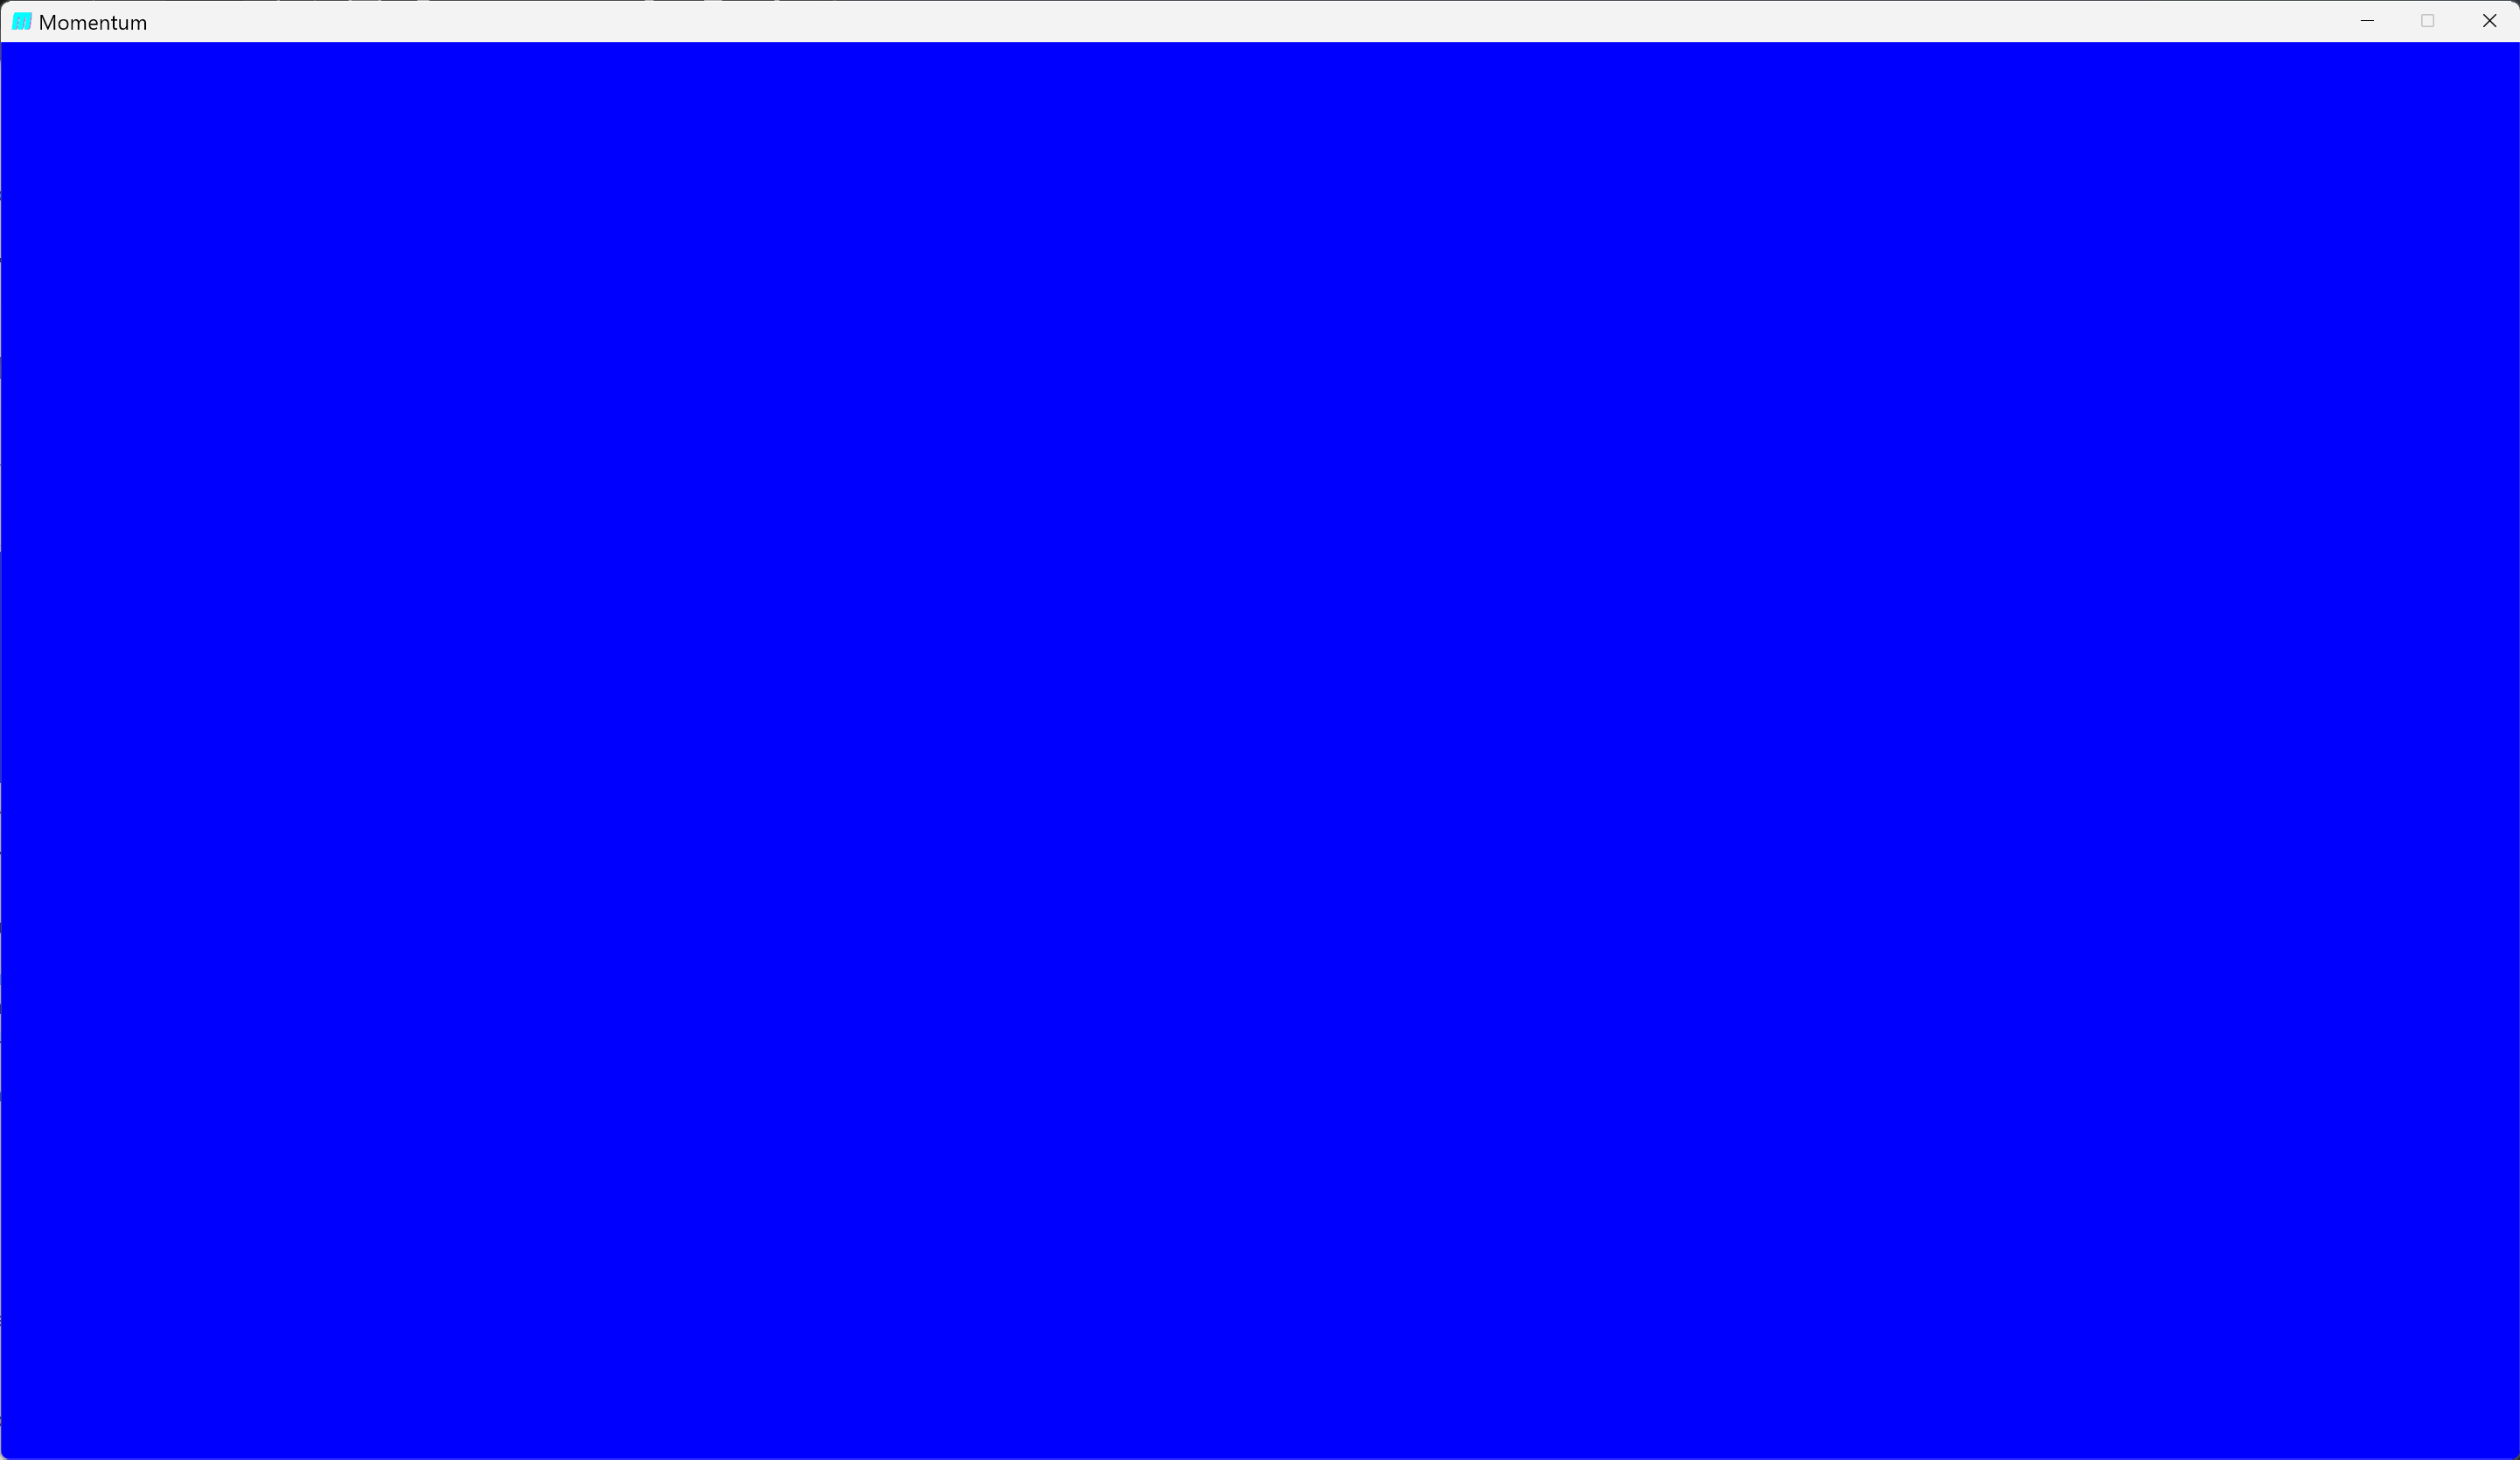
\includegraphics[width = \textwidth]{Development/Images/MenuA.png}
    \caption{Menu A}
    \label{fig:menu_a}
    \end{subfigure}
    \begin{subfigure}{0.49\textwidth}
    \centering
    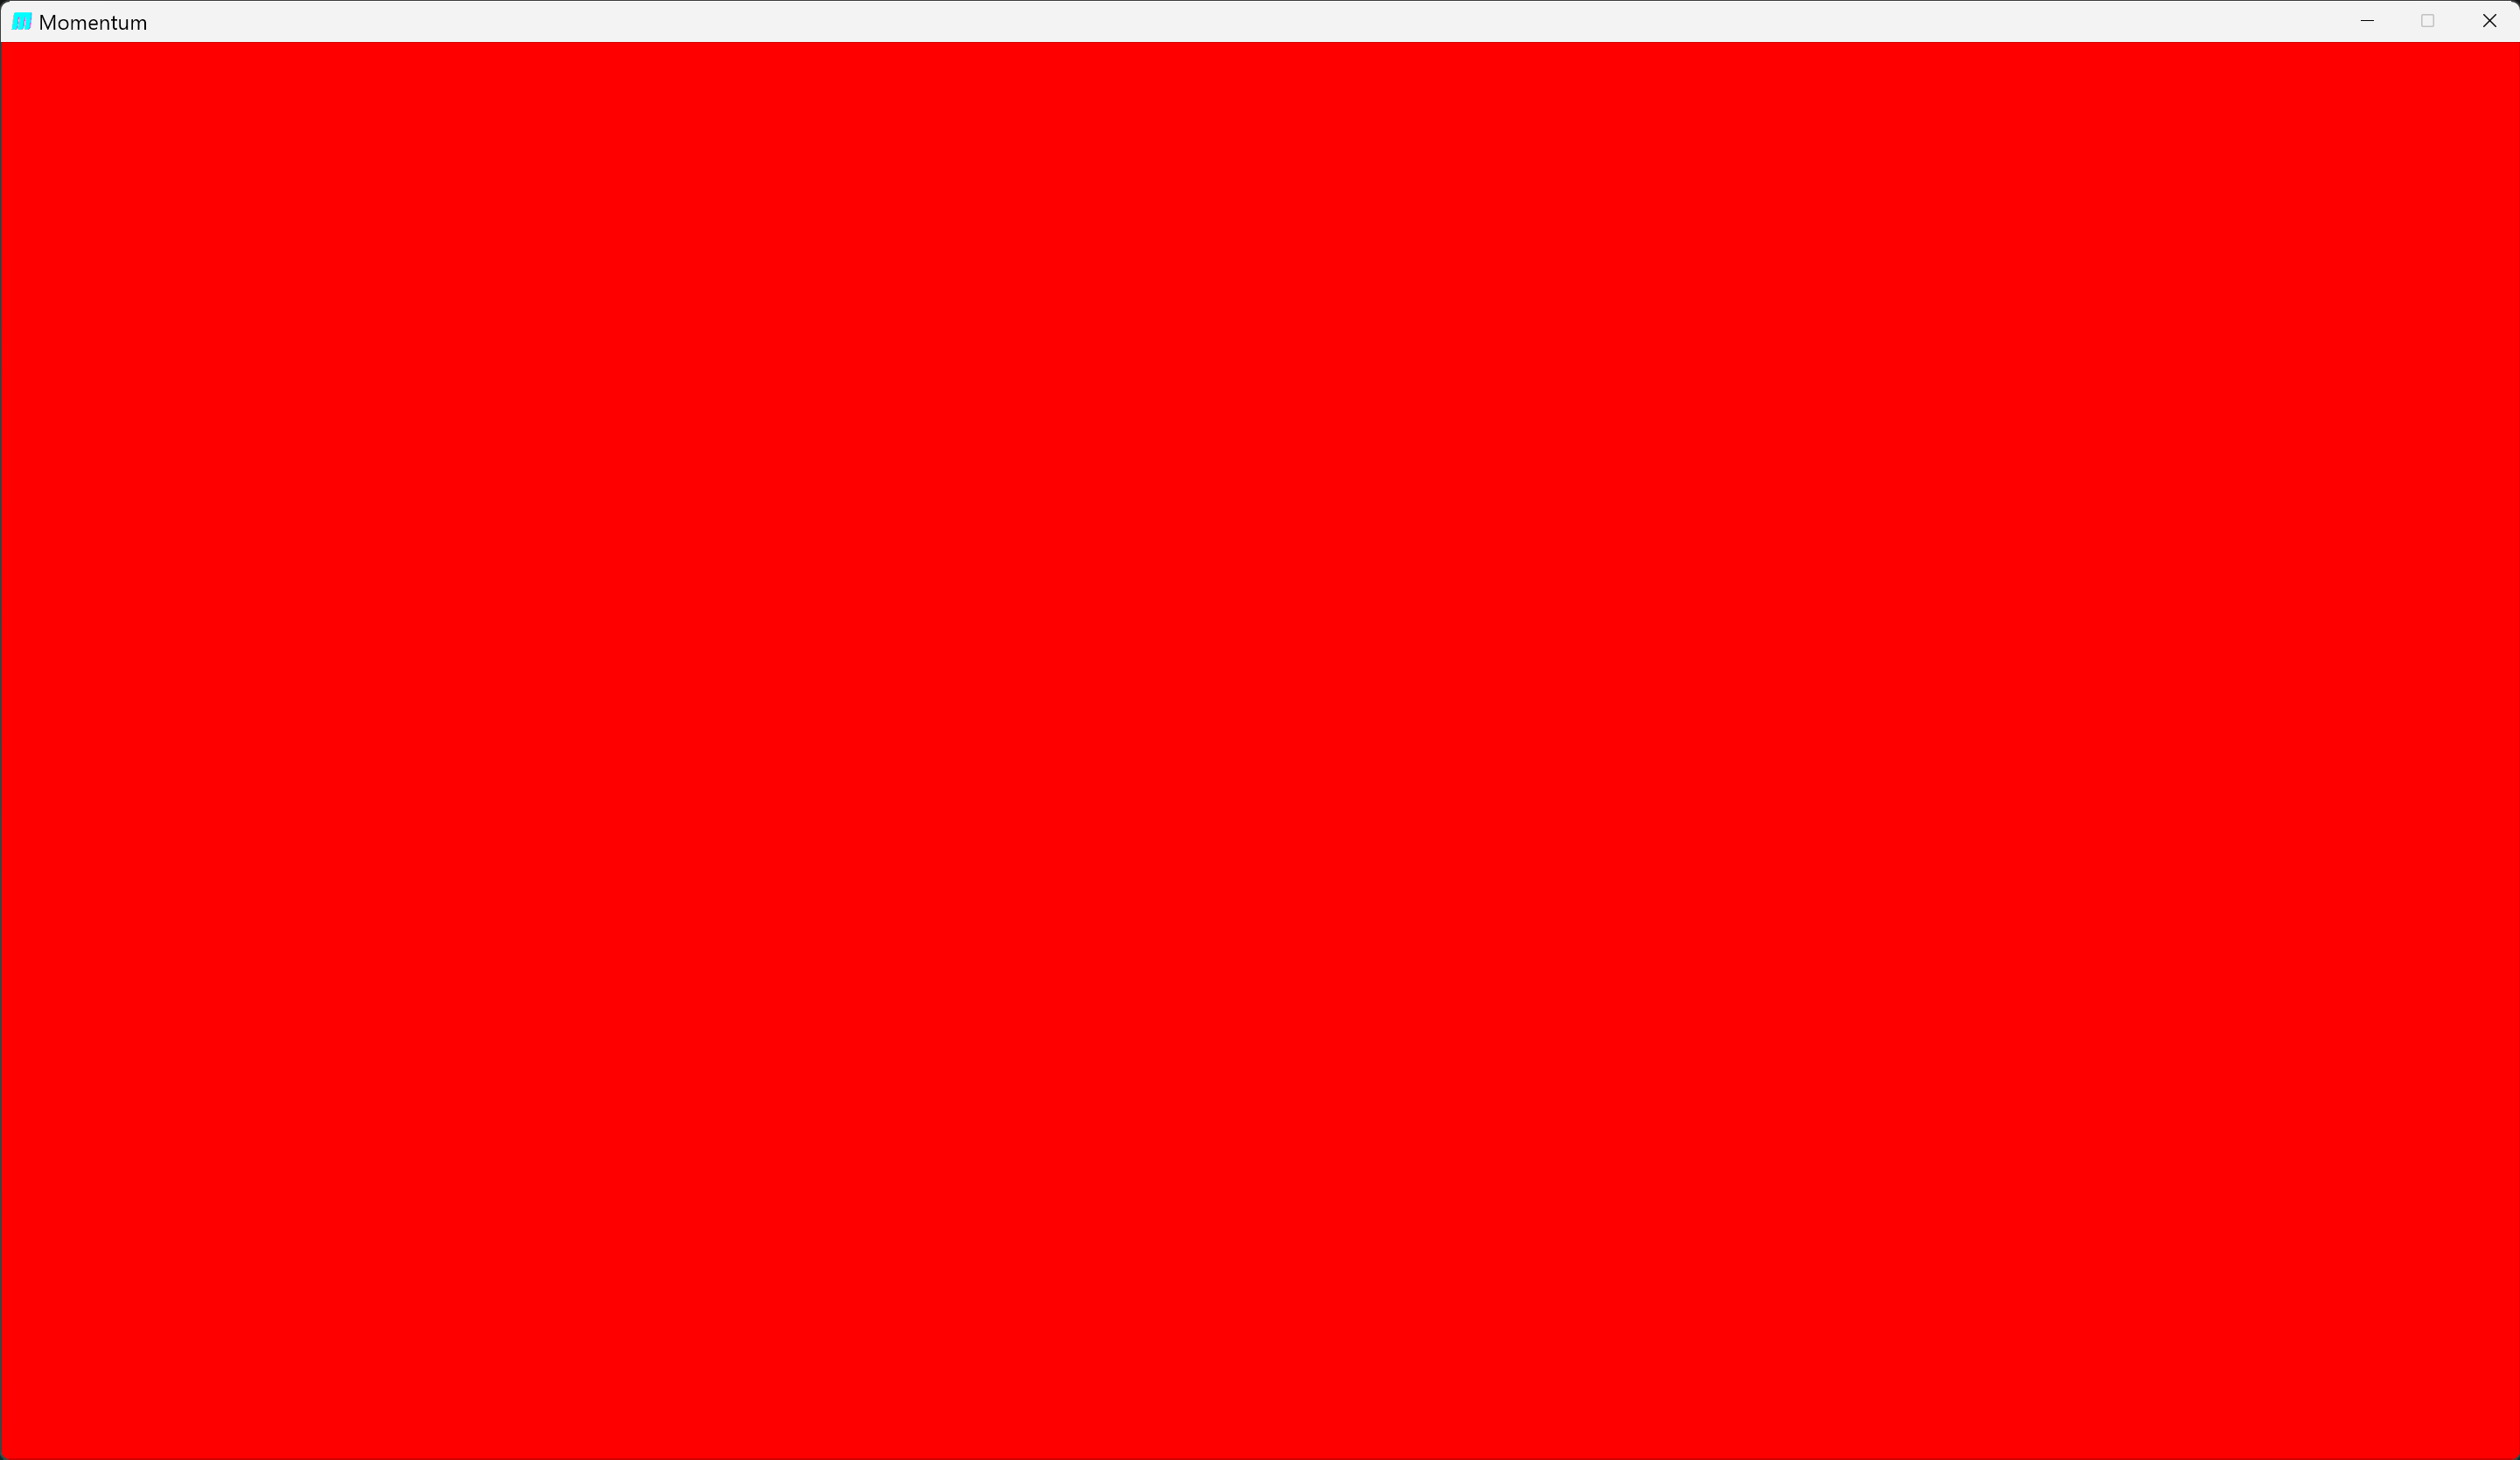
\includegraphics[width = \textwidth]{Development/Images/MenuB.png}
    \caption{Menu B}
    \label{fig:menu_b}
  \end{subfigure}
  \caption{Screen captures from the two menus.}
  \label{fig:menu_ab}
\end{figure}

\vs
We will take the start menu and the login menu to begin with. Each one of these classes will have some text on the screen. We will create the Start Menu first, and then we can show that we can move between them, thus proving that the \m{Game} class works at switching between different states. The first thing we will do is import \m{pygame.FreeType} at the start of \m{menu.py}. We will also create our font object here.


\begin{mpy}
import pygame.freetype

#Initalise freetype
pygame.freetype.init()

#Create text font
text_font = pygame.freetype.SysFont('iosevka', 64)
\end{mpy}

\vs
After this, we need to create our \m{Start} class, which is done as follows. We create our constructor as follows. We need to set our display so that the menu can rende.

\begin{mpy}
#Directed from the login page
class Start:
    def __init__(self, display, gameStateManager):
        #Set the display on which we are rendering
        self.display = display
        
        #Set the gsm
        self.gameStateManager = gameStateManager

        #Set screen dims
        self.SCREEN_DIMS = gameStateManager.SCREEN_DIMS

        #Set bg color
        self.BG_COLOR = (0, 255, 255)
\end{mpy}

\vs
The next part of the code is the running of the menu itself. Here, we will be filling the display with a certain colour, and then writing some text onto it. We set the bounding rectangle to have a centre at the centre of the screen, so that we can align the text nicely. We then check to see if the user wants to quit the game and if not, we repeat the loop until they do. This code was partially constructed with help from \href{https://stackoverflow.com/questions/23982907/how-to-center-text-in-pygame}{this link}.

\vs
\begin{mpy}
  def run(self, returnValues):

    #Fill display
    self.display.fill(self.BG_COLOR)

    #Create clock
    self.clock = pygame.time.Clock()
    dt = 0

    #Initialise variables
    #TODO: SHOULD BE MOVED INSIDE THIS IS A BUG PLEASE DOCUMENT IT
    inPos = False
    running = True
    clicked = False

    #Main loop
    while running:

      #Redraw display
      self.display.fill(self.BG_COLOR)

      #Render text
      text_surface, text_rect = text_font.render('Start Menu', fgcolor=(0, 0, 0), bgcolor=self.BG_COLOR)
      text_rect.center = (self.SCREEN_DIMS[0] // 2, self.SCREEN_DIMS[1] // 2)

      #Blit to surface
      self.display.blit(text_surface, text_rect)

      # Get all events
      events = pygame.event.get()

      # Get all key presses
      keys = pygame.key.get_pressed()
      
      for event in events:

          # Check if user wants to quit
          if event.type == pygame.QUIT:
              pygame.quit()
              sys.exit()

      #Update the display
      pygame.display.update()

      #Tick the clock
      dt = self.clock.tick(self.gameStateManager.REFRESH_RATE)
        
    return returnValues
\end{mpy}

\vs
We also need to change the initial value of the game state manager's state from \m{'game_loop'} to \m{'start'}. Having done this, we get the following image (Figure \ref{start_menu}) on the screen.

\begin{figure}[H]
    \centering
    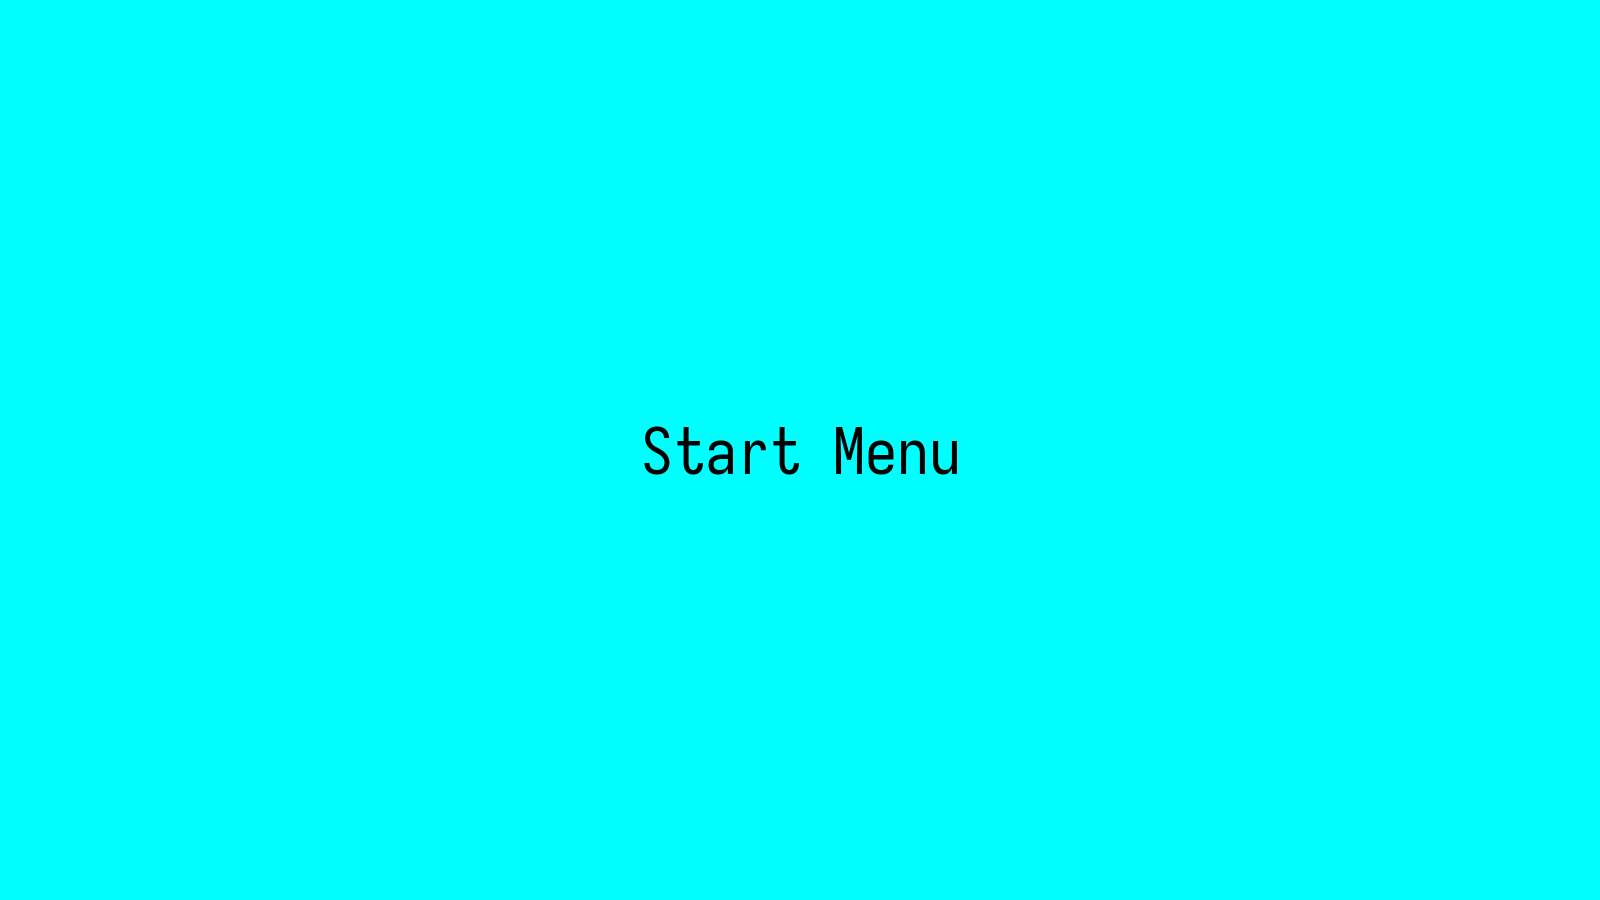
\includegraphics[width=\linewidth]{Development/Images/start_menu.png}
    \caption{An image capture of the start menu screen so far}
    \label{fig:start_menu}
\end{figure}
We can now take inputs from the keyboard and assign actions to them. Specifically, if the user presses a certain button we want to change the state of the \m{GameStateManager} using the setter method and then we want to set the inner loop to stop running so that we can go back to the outer loop and join the new state.

\vs
We can assign the up arrow to be the keyboard event to change the state. This is done as follows.

\begin{mpy}
      if keys[K_UP]:
          self.gameStateManager.setState('game_loop')
          running = False
\end{mpy}

This then means that we can switch to the main game loop immediately after pressing the up arrow key. We will introduce a delay, so that if the holds the arrow key for multiple frames this doesn't cause it to skip through menus. This will prevent them from accidentally skipping through important menus. Alternatively, we could use also use buttons in the menu, and only register when the user has pressed one of the mouse buttons. This will mean that we no longer need to use any delays, since the user will then have likely intentionally clicked on the button that they wanted to click on. Therefore, it would be useful to implement a button class, which we will do later. We will now show a video demonstrating this in action, although the keyboard inputs are not visible. The only input I gave to the system was the up and down arrow keys. However, since we don't have a game loop yet, this is a bit pointless. This is something we will rectify once we have a game loop.

\subsection{\textcolor{red}{Button}}

We will be implementing a \m{Button} class which we mentioned before. This will allow us to more easily use the menu system which we created in the previous section. As mentioned in the Design section, the button is just a rectangle over which we want to check if there has been any clicks. If there has been a click, then we take some action, such as leaving the game, or changing the state. This can be done as follows. We will inherit from the \m{Block} class, since this already implements some important features. Additionally, the \m{Rect} class in \m{PyGame} already implements a collide point method, so we can use that to see whether the position where the mouse has clicked is inside of the rectangle. We will write the constructor as follows.

\begin{mpy}
class Button(Block):

  def __init__(self, centre, length0, length2, colour, SCREEN_DIMS, text, bg_color):
    
    #Middle of the screen
    camera_position = U.mult(SCREEN_DIMS, 0.5)

    #Position as an integer
    camera_position = [int(i) for i in camera_position]

    #Initiate the block class in the 
    super(Button, self).__init__(centre, length0, length2, colour, SCREEN_DIMS, camera_position)

    #Set the bg color
    self.BG_COLOR = bg_color

    #Set the text surface and rect to write on
    self.text_surface, self.text_rect = text_font.render('Start Menu', fgcolor=(0, 0, 0), bgcolor=self.BG_COLOR)

    #Set the centre of the button on the screen
    self.text_rect.center = self.centre

    #Set screen dims for rendering
    self.SCREEN_DIMS = SCREEN_DIMS
\end{mpy}

We set the camera position to be in the middle of the screen, which means that we don't need to adjust our render functions, and we can just use this as our camera position, since we won't be moving anyway.

\vs
We will now write the render function as follows.

\begin{mpy}

  #Modified render function of the button
  def render(self, display, dt):

    #Render the rectange
    super().render(display, U.mult(self.SCREEN_DIMS, 0.5), [0, 0], dt, self.SCREEN_DIMS)

    #Render the text on top
    display.blit(self.text_surface, self.text_rect)
\end{mpy}

\href{https://stackoverflow.com/questions/23982907/how-to-center-text-in-pygame}{This was an important link, and we need to reference it}. We will now change the \m{Start} menu class to make use of this new button. We begin by adding the following lines to the constructor.

\vs
\begin{mpy}
    #Create button instance to use
    self.button = Button(U.mult(self.SCREEN_DIMS, 0.5), 350, 80, self.BG_COLOR, self.SCREEN_DIMS, "hello", self.BG_COLOR)
\end{mpy}

This ensures that we can now use the button object inside of the main loop. However, as of right now, it doesn't have any functionality, so we will implement a click function which will tell us when the mouse cursor is over the button. We can then find when the mouse button is clicked and if both conditions are met then the button has been clicked. In the \m{Button} class we can add a new function.

\tbc


\subsection{\textcolor{blue}{Game Loop}}

We will be creating a new class \m{GameLoop}, which will be running the game loop. To do this, we will be taking the \m{display} which we need to work on, the \m{GameStateManager}, and then we can assign all of the characteristics from this to the class in order to make them even easier to access.
\vs
\begin{mpy}
class GameLoop:

  def __init__(self, display, gameStateManager):

    #Get the display we are working on
    self.display = display

    #Get the gameStateManager, so we can process it within the class
    self.gameStateManager = gameStateManager

    #Get the screen dimensions conveniently
    self.SCREEN_DIMS = self.gameStateManager.SCREEN_DIMS
\end{mpy}

\vs
We also need to initialise a new clock and set \m{dt} in order to be able to use frame-rate independent physics. We have currently set a place holder on the initial position of the player until we set up spawn points, teams, etc.

\vs

\begin{mpy}
    #Placeholders for the moment
    self.pos_x = self.SCREEN_DIMS[0]//2
    self.pos_y = self.SCREEN_DIMS[1]//2

    #Initialise the clock, and set the refresh rate
    self.clock = pygame.time.Clock()
    self.REFRESH_RATE = self.gameStateManager.REFRESH_RATE
\end{mpy}
\vs
We need to create an actual game loop. Specifically, we need to contain this game loop inside of a run function, since all of the game state objects will contain a \m{run()} function that will be called everytime we are changing states. 
\begin{mpy}
  def run(self, returnValues):

    dt = 0

    player1 = Player([self.pos_x, self.pos_y], [0, -1], 0, 'empty')

    #List of all players
    self.players = [player1]

    running = True

    while running:

      self.display.fill((255, 255, 255))

      #Check if player wants to quit
      for event in pygame.event.get():
        if event.type == pygame.QUIT:
          pygame.quit()
          sys.exit()

      #Get the key presses and mouse position and buttons
      keys = pygame.key.get_pressed()

      mouse_pos = pygame.mouse.get_pos()

      mouse_clicks = pygame.mouse.get_pressed()

      #Get direction vector
      player1_direction = [mouse_pos[0] - self.SCREEN_DIMS[0]//2, mouse_pos[1] - self.SCREEN_DIMS[1]//2]

      #Normalise direction vector
      dir_mag = sqrt(sum([i**2 for i in player1_direction]))
      player1_direction = [i / dir_mag for i in player1_direction]

      #Update the direction vector
      player1.forward_vec = player1_direction

      #Get the directions which are pressed
      directions = [int(keys[K_d]), int(keys[K_a]), int(keys[K_s]), int(keys[K_w])]

      for player in self.players:
          player.render(self.display, player1.position, directions, dt, self.SCREEN_DIMS)

      #Update the display
      pygame.display.update()

      #Tick the clock
      dt = self.clock.tick(self.REFRESH_RATE)/1000

    return None
\end{mpy}

We will now re-write the \m{render()} function in the \m{Player} class, since there is a lot of ineffecienies in the way it was written, and now that the \m{Utility} class is available we can make the code a lot more efficient, readable, and maintainable. Additionally, there were a lot of values that were being calculated twice, and now we can get rid of that. This produces the following code.
\vs

\begin{mpy}
  #Renders the character to the display of the player
  def render(self, display, camera_position, directions, dt, SCREEN_DIMS):

    #Find relative posistion
    rel_pos = U.convertToScreen(camera_position, self.position, SCREEN_DIMS)

    #Draw the circle
    pygame.draw.circle(display, self.colour, rel_pos, self.radius)

    #Final extent of the forward vector
    for_pos = U.vecAdd(U.mult(self.forward_vec, 100), rel_pos)

    #Draw anti-aliased line for forward vector
    pygame.draw.aaline(display, (0, 0, 0), rel_pos, for_pos)

    #Move the player
    self.movePlayer(directions, dt)
\end{mpy}



Setting the start state to be \m{"game_loop"}, we can only see a blank screen. This is because we aren't drawing anything to the screen. Therefore, we need to add the \m{render()} function to the main loop. Whilst we are doing that, we can also add a block, since the player will just be stationary in the middle of the screen. We start by adding the block to the section before the \m{while} loop in the \m{run()} function.

\begin{mpy}
    block1 = Block([self.pos_x, self.pos_y + 200], 100, 200, (100, 0, 0), self.SCREEN_DIMS, player1.position)

    #List of all blocks
    blocks = [block1]
\end{mpy}

Then, we add the following lines of code in the \m{while} loop, as shown below. The first and last lines are already present, but were added for clarity. This will now render both the player and the block.

\begin{mpy}
      #Get the directions which are pressed
      directions = [int(keys[K_d]), int(keys[K_a]), int(keys[K_s]), int(keys[K_w])]

      for player in players:
        player.render(self.display, player1.position, directions, dt, self.SCREEN_DIMS)

      for block in blocks:
        block.render(self.display, player1.position, directions, dt, self.SCREEN_DIMS)

      #Update the display
      pygame.display.update()
\end{mpy}

This results in the output shown below.

\begin{figure}[H]
    \centering
    {
    \setlength{\fboxsep}{0pt}%
    \setlength{\fboxrule}{1pt}%
    \fbox{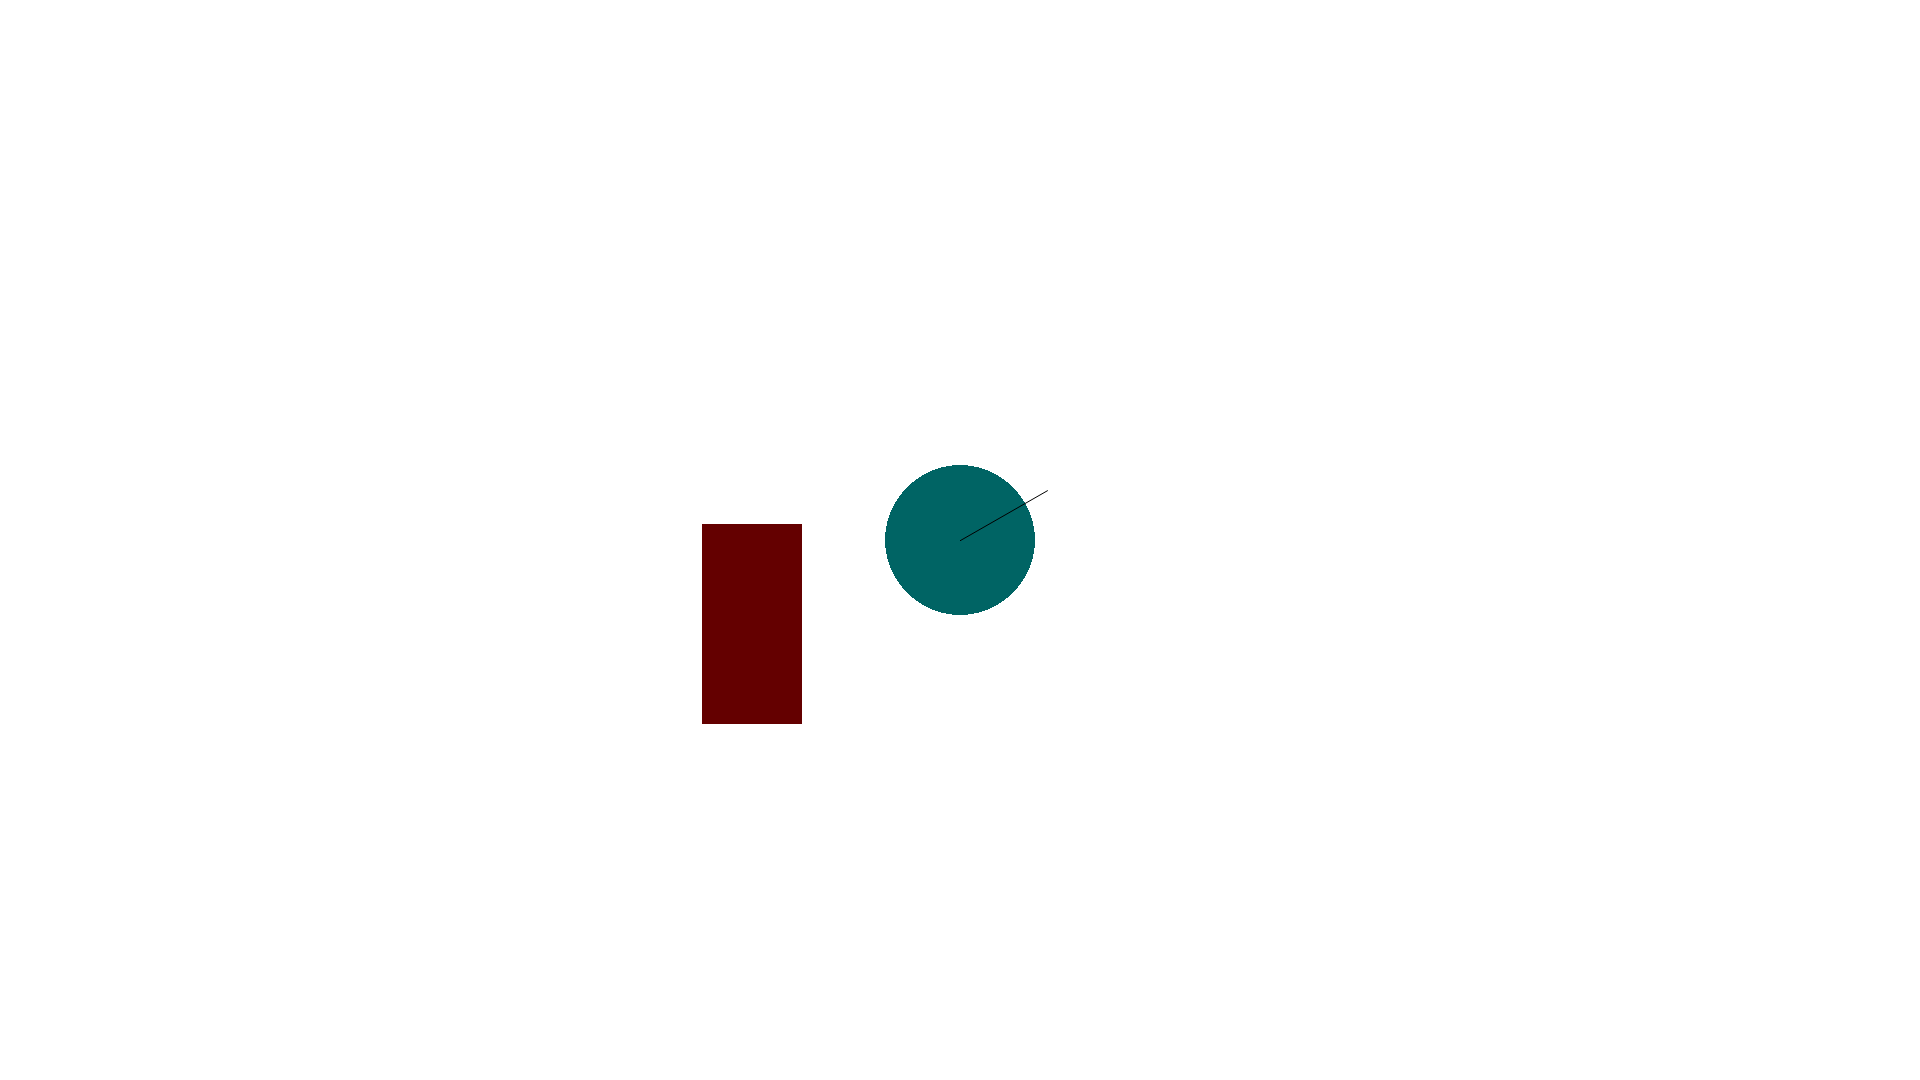
\includegraphics[width=\linewidth]{Development/Images/game_loop_1.png}}
    }
    \caption{An image capture of the game loop}
    \label{fig:game_loop_1}
\end{figure}

Here is a \href{https://youtu.be/ICvIX3ar_eY}{video} demonstrating what this looks like. Both keyboard and mouse inputs were given here.

\vs
We can now add more players and more blocks into the map in order to make the game loop more alike to a real game setting. This is done simply by adding more player instances at different positions. For now, we will set the players to be in the top left corner of the map, and at regularly space intervals. We also want to be able to differentiate between the two teams, so we add this bit of code into the constructor for \m{Player}. This will allow us to choose colours based on which team the player is in.

\begin{mpy}
    self.colours = {0: (0, 100, 100),
                    1: (100, 20, 0)
                    }

    self.colour = self.colours[team]
\end{mpy}

Now that we have this, we can add the players as follows.

\begin{mpy}
    # Team 1
    player1 = Player([self.pos_x - 500, self.pos_y + 400], [0, -1], 0, Shotgun())
    player2 = Player([self.pos_x, self.pos_y + 400], [0, -1], 0, AssaultRifle()
    )
    player3 = Player([self.pos_x + 500, self.pos_y + 400], [0, -1], 0, SniperRifle()
    )

    # Team 2
    player4 = Player([self.pos_x - 500, self.pos_y], [0, 1], 1, Shotgun())
    player5 = Player([self.pos_x, self.pos_y], [0, 1], 1, AssaultRifle())
    player6 = Player([self.pos_x + 500, self.pos_y], [0, 1], 1, SniperRifle())

    # Contains all of the players in the game
    self.players = [player1, player2, player3, player4, player5, player6]
\end{mpy}

We will temporarily remove the block from the scene, and add it back later. We still need to make one more change however. Since the other players will be controlled with AI, we need to find some way of getting inputs to the other players. To do this, we will be using a list containing all of the inputs to the other players. We will set one of these inputs to be the human input, which will then control \m{player1}. To do this efficiently, we will use the \m{enumerate} keyword in \m{Python}. This is written as follows.

\begin{mpy}
      #Output from the model will go here
      model_predictions = [
        directions,
        [0, 0, 0, 0],
        [0, 0, 0, 0],
        [0, 0, 0, 0],
        [0, 0, 0, 0],
        [0, 0, 0, 0],
      ]

      #Render and move players as needed
      for i, player in enumerate(players, 0):
        player.render(self.display, player1.position, model_predictions[i], dt, self.SCREEN_DIMS)
\end{mpy}

This appears as shown in Figure \ref{fig:game_loop_2}. \href{https://youtu.be/KU45hIX5U_0}{Here is a video} showing this in action.

\begin{figure}
  \centering
  \begin{subfigure}{0.49\textwidth}
    \centering
    {
    \setlength{\fboxsep}{0pt}%
    \setlength{\fboxrule}{1pt}%
    \fbox{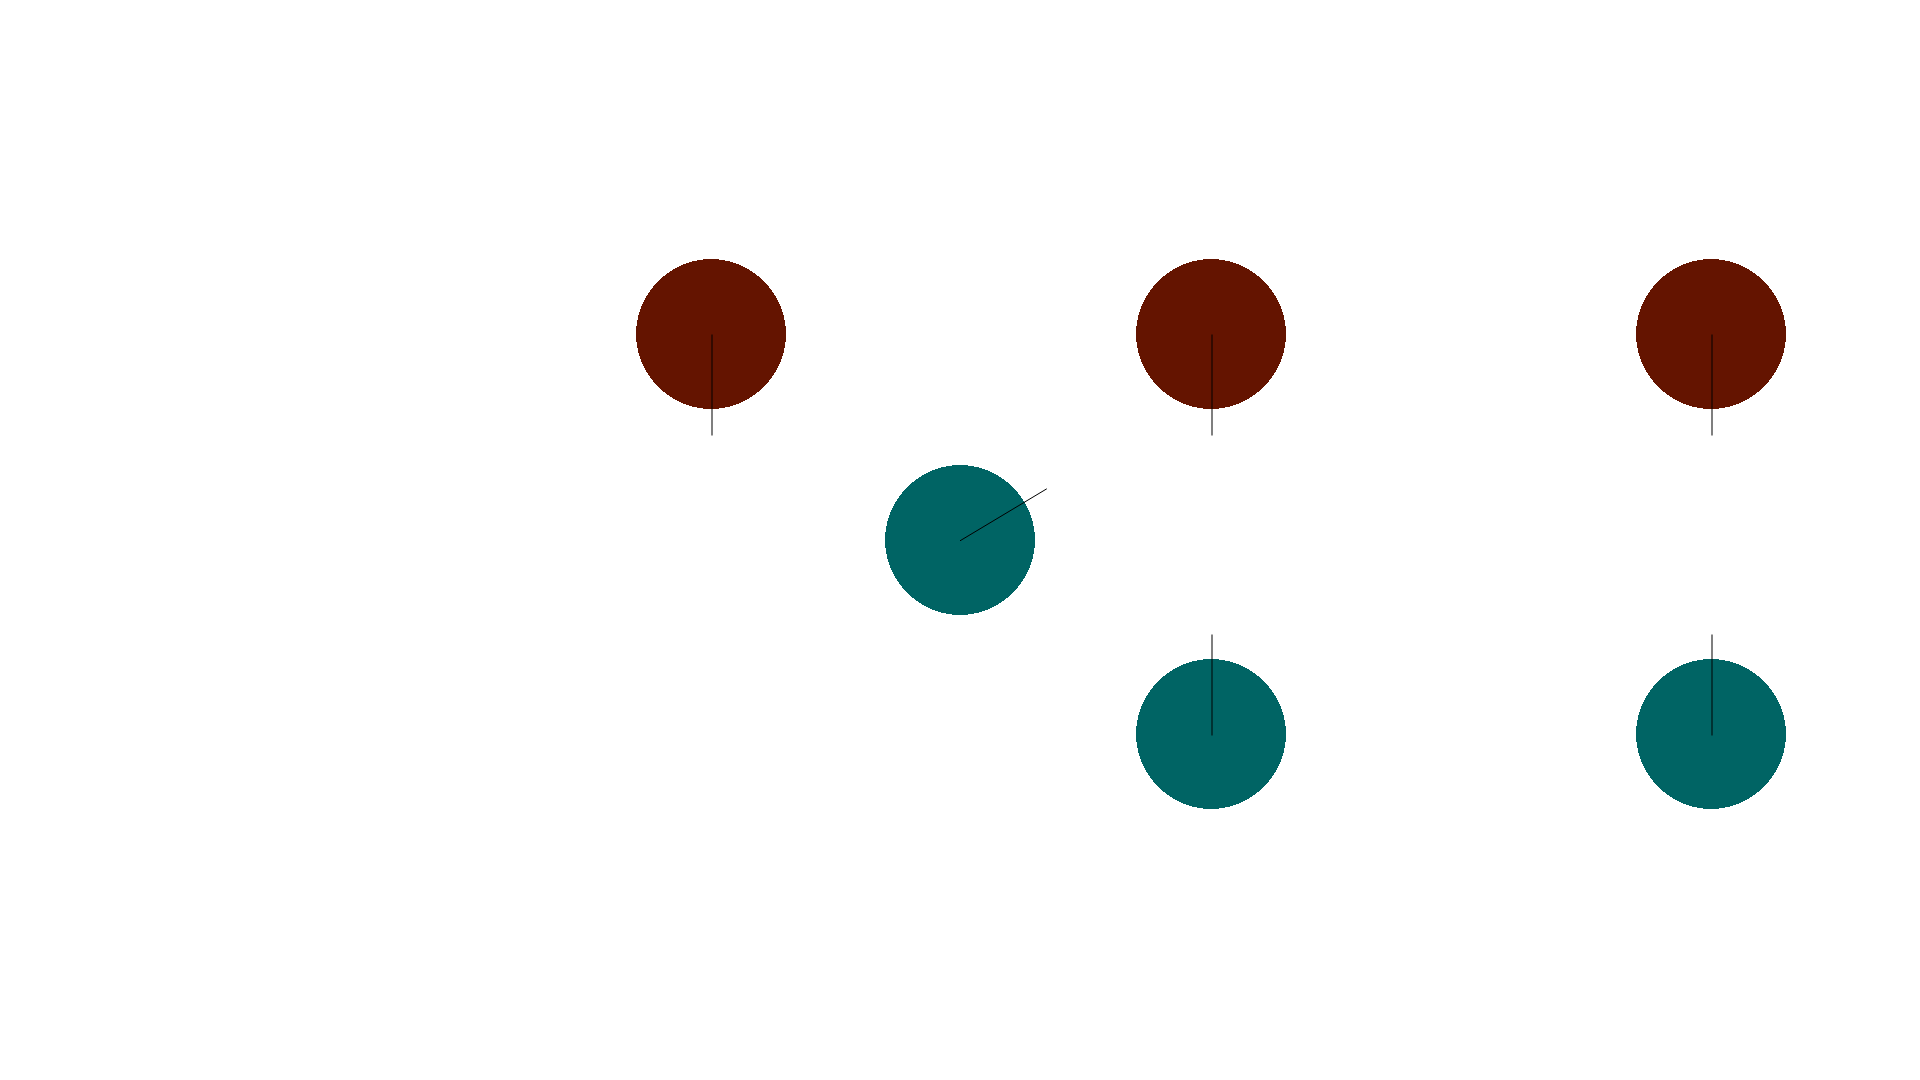
\includegraphics[width = \textwidth]{Development/Images/game_loop_2.png}}}
    \caption{Screen Capture 1}
    \label{fig:game_loop_2_1}
    \end{subfigure}
    \begin{subfigure}{0.49\textwidth}
    \centering
    {
    \setlength{\fboxsep}{0pt}%
    \setlength{\fboxrule}{1pt}%
    \fbox{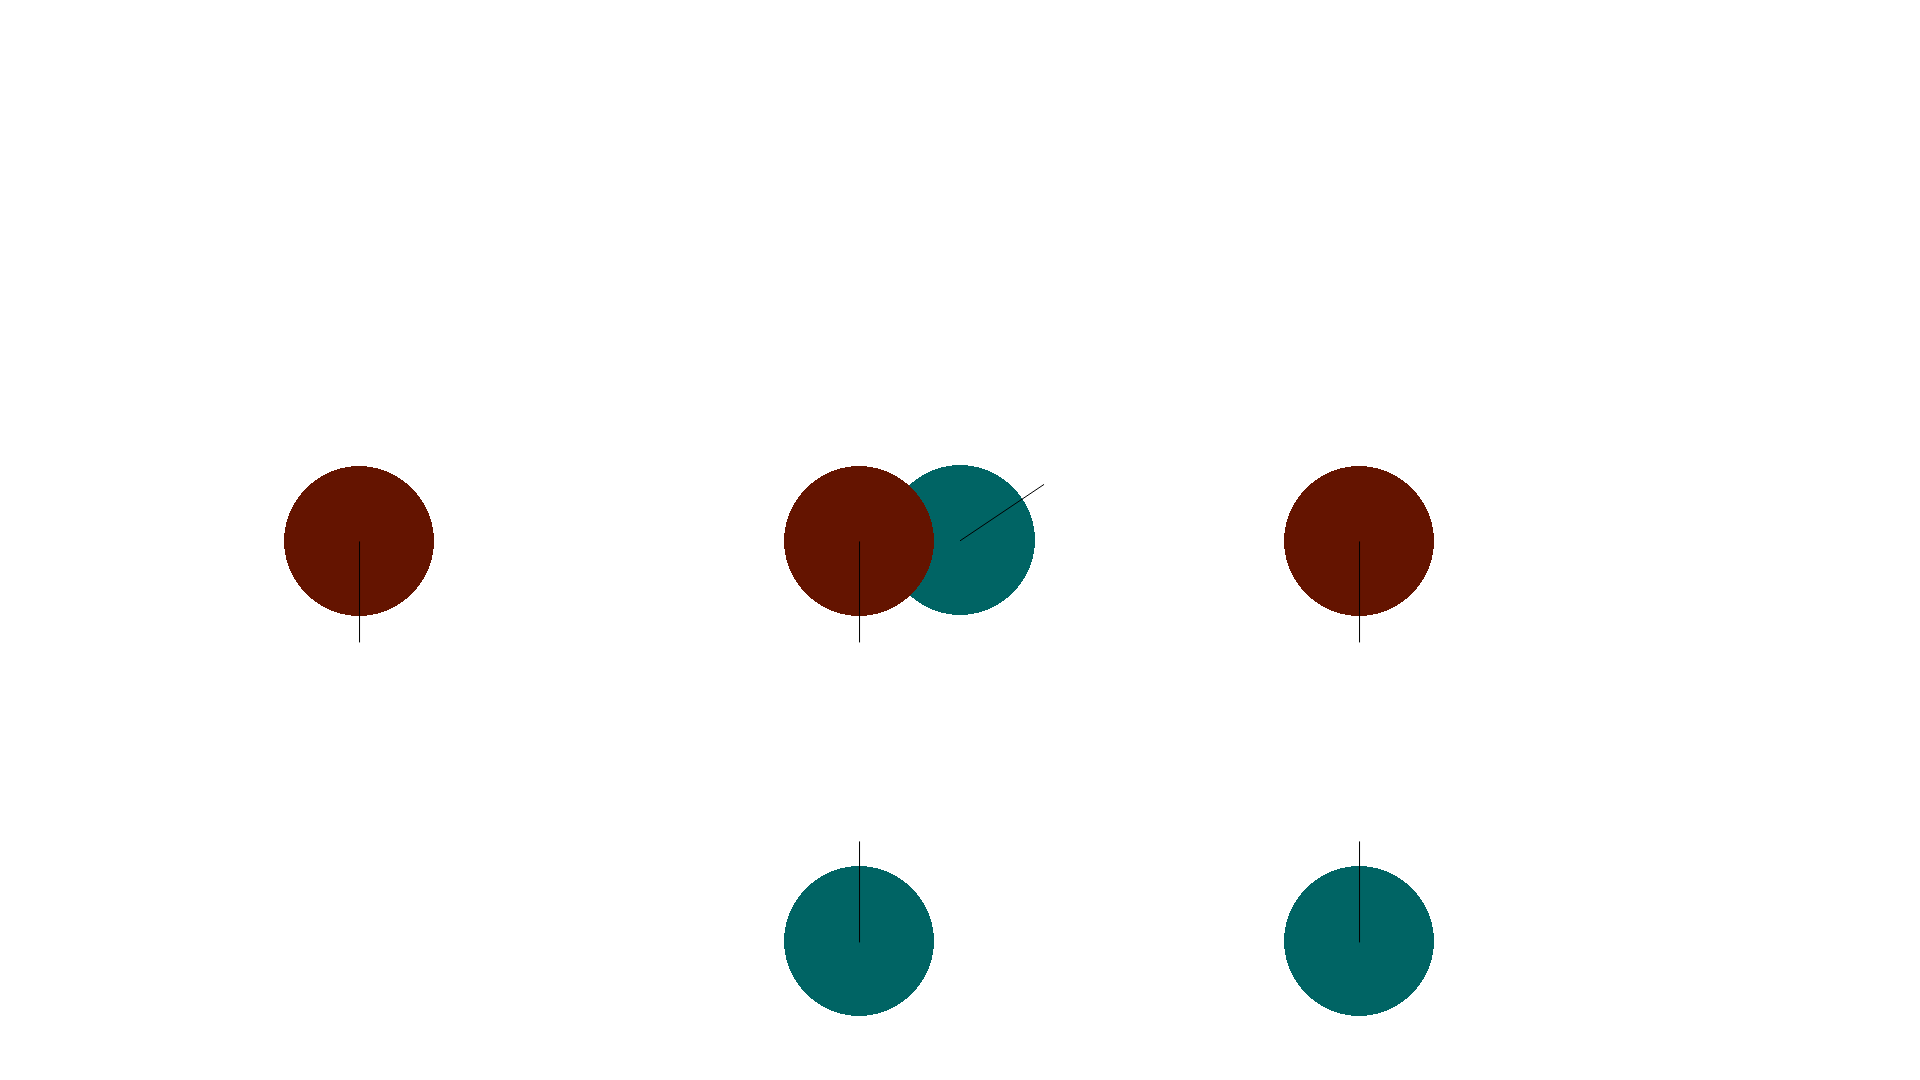
\includegraphics[width = \textwidth]{Development/Images/game_loop_2_b.png}}}
    \caption{Screen Capture 2}
    \label{fig:game_loop_2_2}
  \end{subfigure}
  \caption{Screen captures of two different states in the game loop.}
  \label{fig:game_loop_2}
\end{figure}

\vs
Then next thing we need to do is seperate the render function and the player update. This is important because we need to be able to manage the player states instead of moving it directly. Additionally, it is not the responsibility of the render function to do this. Therefore, we will create a new \m{updatePlayerState} which will take in the directions, and will update the player states.

\begin{mpy}
  def updatePlayerState(self, action, dt):
    #Move the player
    self.movePlayer(action, dt)
\end{mpy}

We will now remove the \m{directions} and \m{dt} inputs from the \m{render()} function since they are no longer needed. This gives the same outputs as shown above. Furthermore, we want to now change the way we are taking inputs. This is because they are based on convention and will make the output from the models harder to work with. Additionally, when we start working with the AI, it is difficult to get an output for the forward and backwards directions and similarly for horizontal inputs, since it is much easier to work with just a single value between -1 and 1. Therefore, we will update the move player function as follows.

\begin{mpy}
  def movePlayer(self, directions, dt):
    #directions = [horizontal input, vertical input]

    #Used to normalise directions
    magnitude = sqrt(U.dot(directions, directions))

    #If no movement, break
    if magnitude == 0:
        return None

    #Calculate movement in the frame
    frameMovement = U.mult(directions, (dt * self.max_speed)/magnitude)

    #Update position
    updatedPosition = U.vecAdd(self.position, frameMovement)

    #Position must be inside of the field
    for i in range(2):
        
      if updatedPosition[i] - self.radius <= 0:
        updatedPosition[i] = self.radius

      elif updatedPosition[i] + self.radius >= 8000:
        updatedPosition[i] = 8000 - self.radius

    #Set new position
    self.position = updatedPosition
\end{mpy}

However, there is still a problem with this code. This is because, if we put our input into the red team, we see that the inputs are still moving the same way they would for the blue team. This is shown in this \href{https://youtu.be/XTUu_KktHLQ}{video}.

However, this is not what we expect to see. The way to resolve this is to use the initial forward vector of the player. This is done as follows. We need to start by creating a right pointing vector in the constructor.

\begin{mpy}
    if self.initial_forward_vec == [0, -1]:
      self.initial_right_vec = [1, 0]
    else:
      self.inital_right_vec = [-1, 0]
\end{mpy}

However, there is still a more efficient way of doing this. The inputs are completely flipped for the opposite team, so we just need to multiply the input direction by -1 for the red team, and for 1 on the blue team. We can remove the right vector, since it is no longer required. We can add the following lines in the constructor.

\begin{mpy}
    if self.initial_forward_vec == [0, -1]:
      self.movement_multiplier = 1
    else:
      self.movement_multiplier = -1
\end{mpy}

Then, the movement is updated as follows.

\begin{mpy}
    #Calculate movement in the frame
    frameMovement = U.mult(directions, self.movement_multiplier * dt * self.max_speed/magnitude)
\end{mpy}

This then produces the output we expect, as shown \href{https://youtu.be/ZixPY08tVlE}{in this video}.
\vs

The model will output a dictionary of the inputs that it wants the player to take. Therefore, we will modify our code as follows. In the \m{run()} function, we want to edit the \m{model_predictions} to be as follows.

\begin{mpy}
      #Output from the model will go here
      model_predictions = [
        {"forward": directions[1], "right": directions[0], "rot_rate": 0},
        {"forward": 0, "right": 0, "rot_rate": 0},
        {"forward": 0, "right": 0, "rot_rate": 0},
        {"forward": 0, "right": 0, "rot_rate": 0},
        {"forward": 0, "right": 0, "rot_rate": 0},
        {"forward": 0, "right": 0, "rot_rate": 0},
      ]
\end{mpy}

In the \m{updatePlayerState()}, we do the following.

\begin{mpy}
  #Update the player state
  def updatePlayerState(self, action, dt):

    #Get the directions from the dictionary
    directions = [action["right"], action["forward"]]

    #Move the player
    self.movePlayer(directions, dt)
\end{mpy}

In the \m{run()} we also need to update the player state as follows. We will do this in a seperate loop, because we will also need to do state updates between the player movement update and the rendering.

\begin{mpy}
      #Update player states
      for i, player in enumerate(players, 0):
        player.updatePlayerState(model_predictions[i], dt)
\end{mpy}

We also need to rotate the direction vector. This is done as follows using the \m{U.rotateVec()} method we defined before. This is inserted into \m{updatePlayerState()}.

\begin{mpy}
    #If dt != 0 we want to turn
    if dt != 0:
      angleTurned = action["rot_rate"] * dt
      self.forward_vec = U.rotateVector(self.forward_vec, angleTurned)
\end{mpy}

We will also change the rotation rate for some of the characters. This will allow us to this in action.

\begin{mpy}
      #Output from the model will go here
      model_predictions = [
        {"forward": directions[1], "right": directions[0], "rot_rate": 0},
        {"forward": 0, "right": 0, "rot_rate": 1.5},
        {"forward": 0, "right": 0, "rot_rate": -1},
        {"forward": 0, "right": 0, "rot_rate": 1},
        {"forward": 0, "right": 0, "rot_rate": -1},
        {"forward": 0, "right": 0, "rot_rate": 0},
      ]
\end{mpy}

This produces the output as shown in Figure \ref{fig:game_loop_3_rot}, and also in \href{https://youtu.be/GxHD5rflfGw}{this video}.

\begin{figure}
  \centering
  \begin{subfigure}{0.49\textwidth}
    \centering
    {
    \setlength{\fboxsep}{0pt}%
    \setlength{\fboxrule}{1pt}%
    \fbox{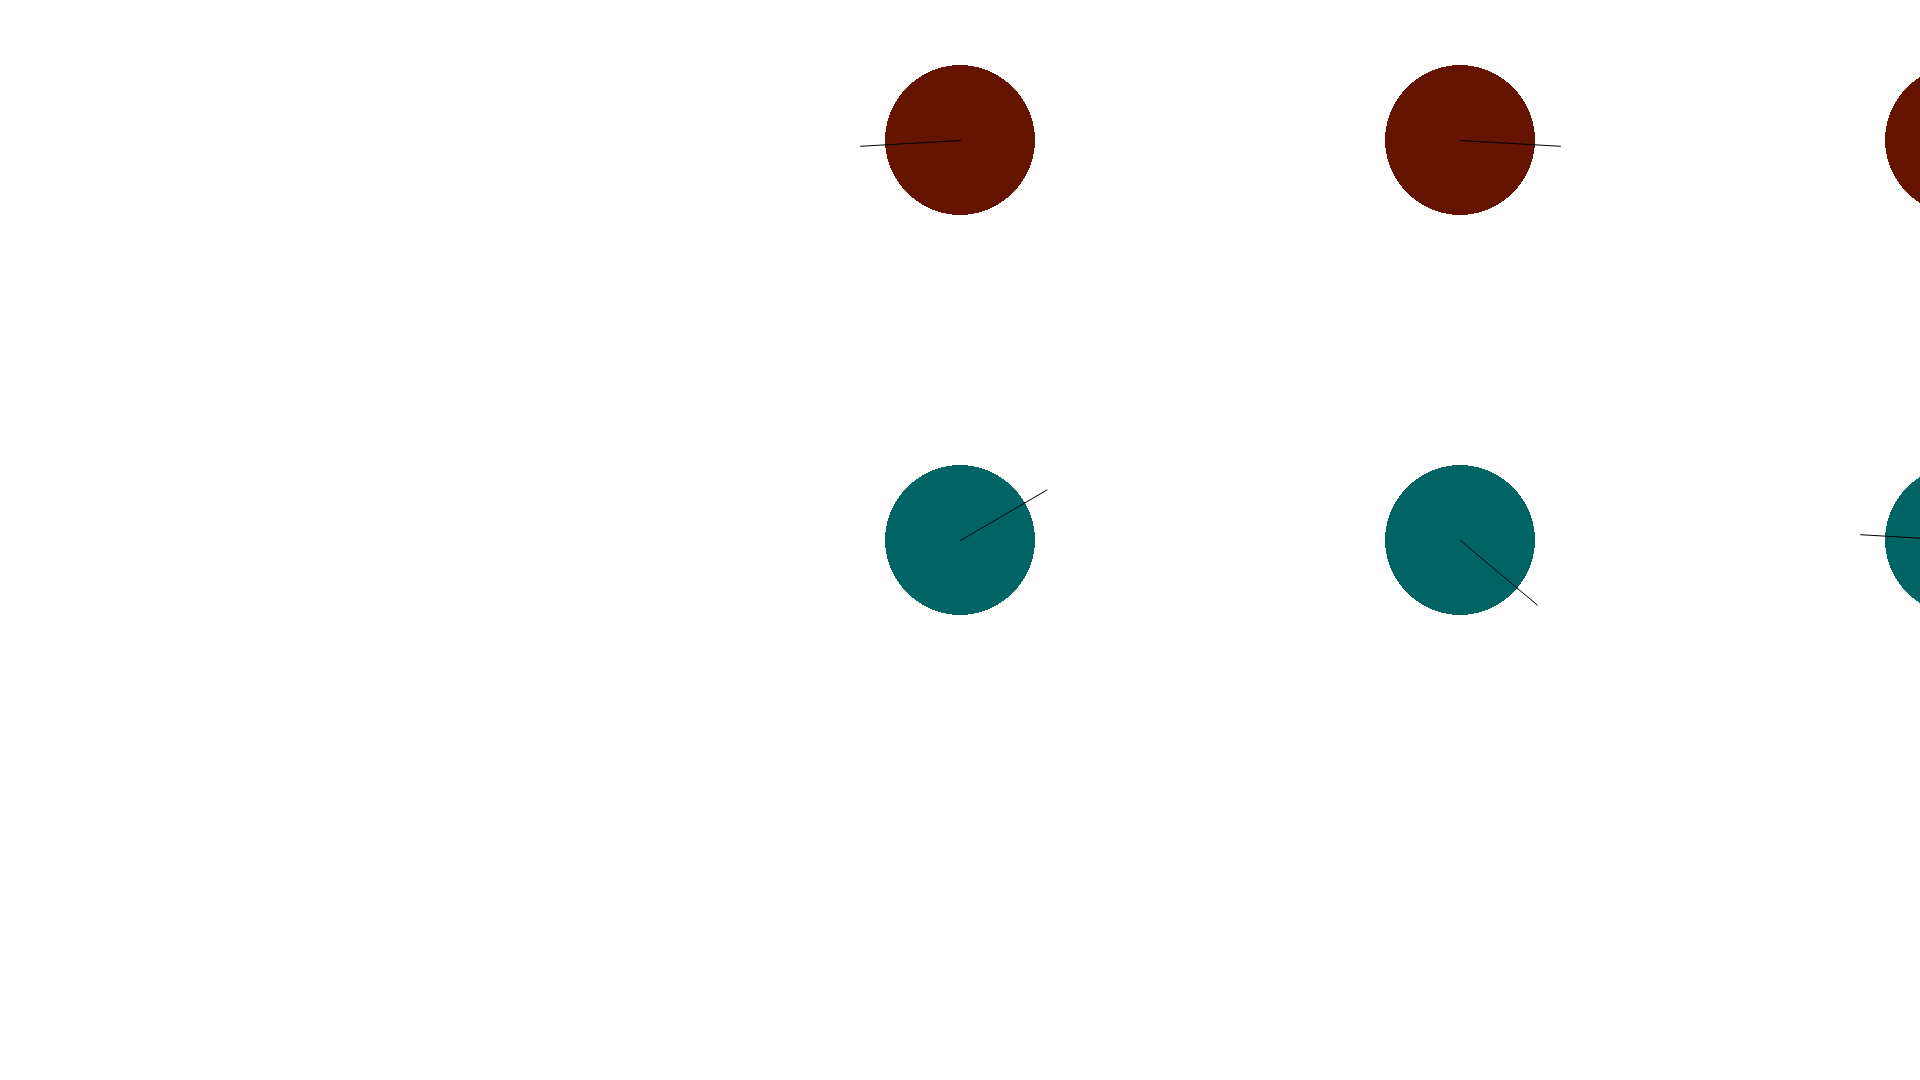
\includegraphics[width = \textwidth]{Development/Images/game_loop_3_a.png}}}
    \caption{Screen Capture 1}
    \label{fig:game_loop_3_1}
    \end{subfigure}
    \begin{subfigure}{0.49\textwidth}
    \centering
    {
    \setlength{\fboxsep}{0pt}%
    \setlength{\fboxrule}{1pt}%
    \fbox{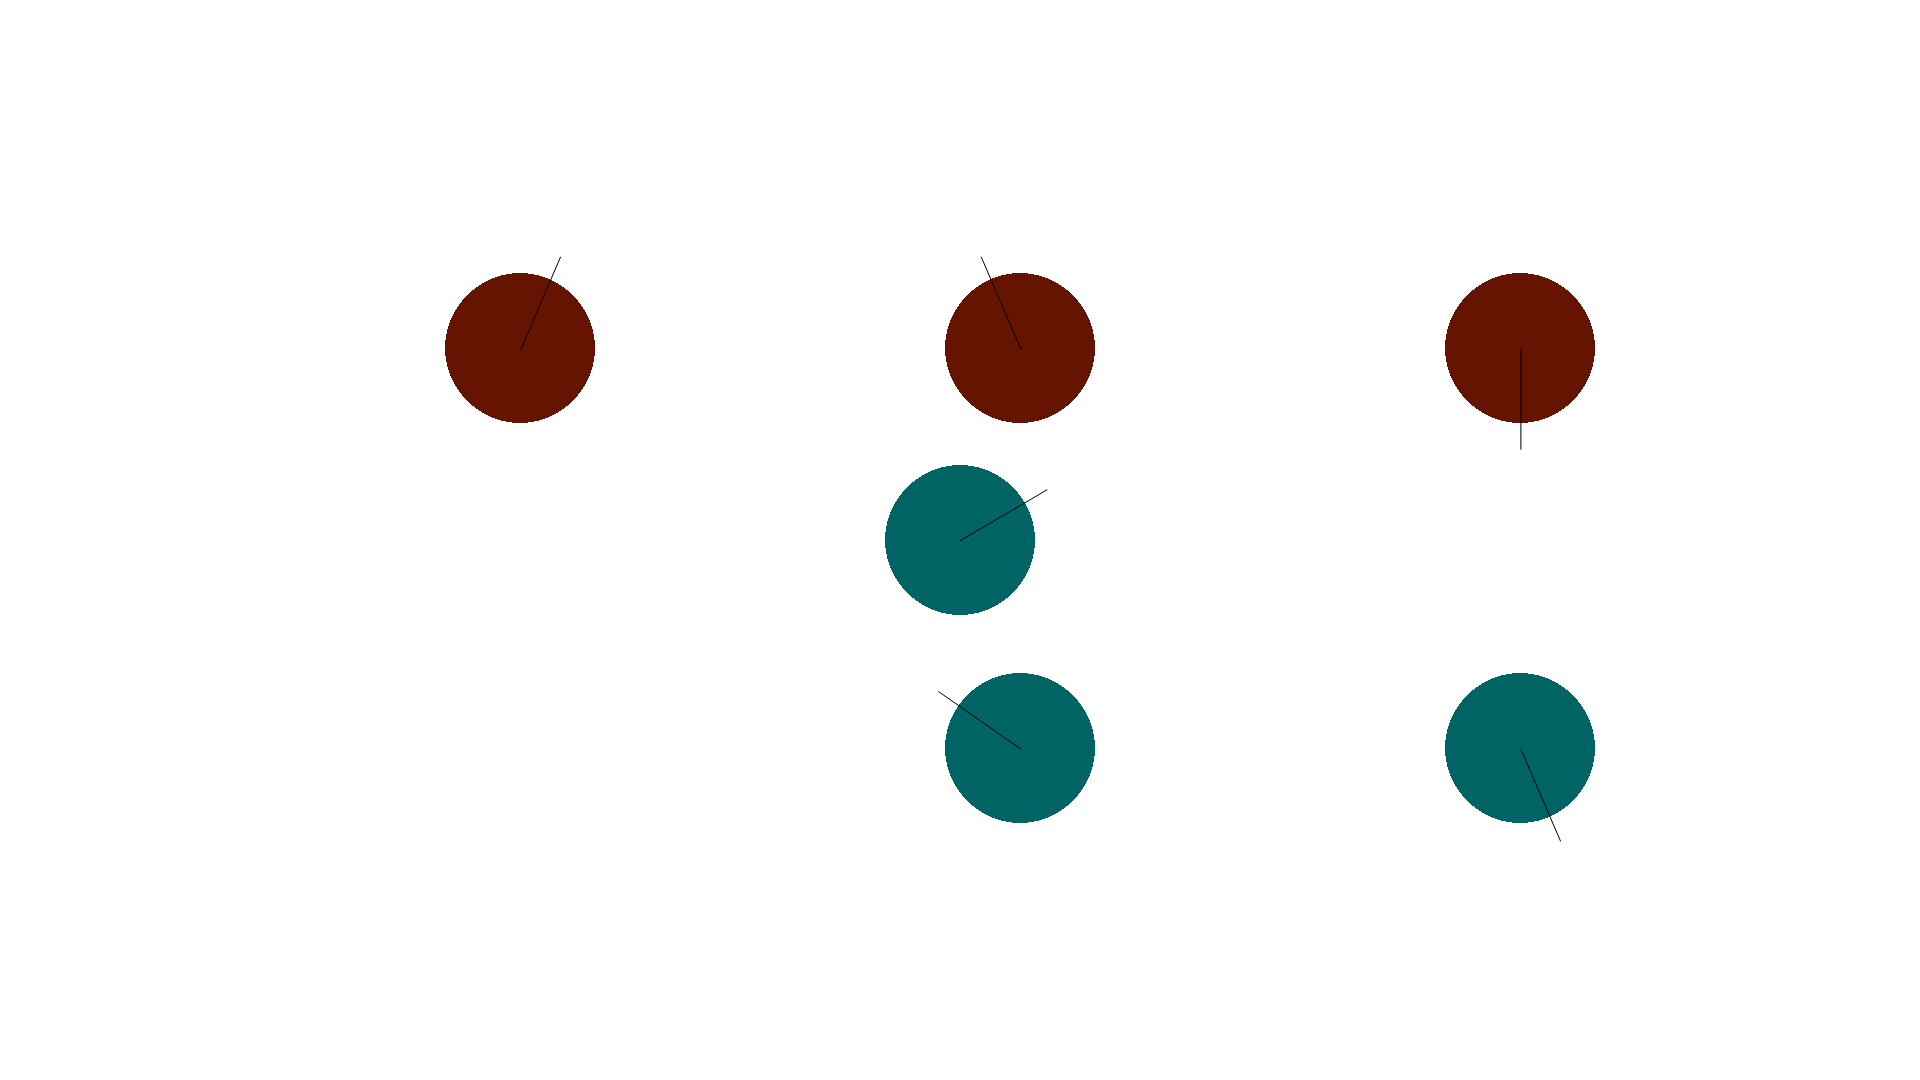
\includegraphics[width = \textwidth]{Development/Images/game_loop_3_b.png}}}
    \caption{Screen Capture 2}
    \label{fig:game_loop_3_2}
  \end{subfigure}
  \caption{Screen captures of two different states in the game loop whilst the players are rotating.}
  \label{fig:game_loop_3_rot}
\end{figure}

The next thing we want to do is to implement the firing system. This is the primary mechanic in the game, so it is important to implement it. To do this, we will need to setup a few things. Firstly, we need to take inputs for whether the player is firing or not. We can do this using another key in the inputs dictionary. We can also add an extra line in the \m{updatePlayerState()} to account for this. This is done as follows.
\begin{mpy}
    #Array of [Position, Final Extent, Damage]
    if action["firing"]:
      weaponRay = self.fire()
    else:
      weaponRay = []

    return weaponRay
\end{mpy}

We have not accounted for the cooldown of the weapon yet, but this is something we will implement in the next iteration of the weapon system. For now, we will need to update the main \m{run()} function. This is done as follows.

\begin{mpy}
      rays = {}
      #Update player states
      for i, player in enumerate(players, 0):
        rays[player] = player.updatePlayerState(model_predictions[i], dt)
\end{mpy}

We will also create a new function \m{handlesRayCollisions()} to deal with all of the rays that are being fired.

\begin{mpy}

\end{mpy}

In order to make the damage on the players more clear, we can display the health of the player on them. This will make the code easier to debug, and will show the player the health of the enemy. We add the following code to the start of the \m{player.py} file.

\begin{mpy}
import pygame.freetype

pygame.freetype.init()
text_font = pygame.freetype.SysFont('iosevka', 48)
\end{mpy}

In the render function, we add the following lines at the end.

\begin{mpy}
        #Create text surface of the health
        self.text_surface, self.text_rect = text_font.render(str(self.health), fgcolor=(255,255,255), bgcolor=self.colour)

        #Set text position
        self.text_rect.center = rel_pos

        #Blit the text
        display.blit(self.text_surface, self.text_rect)
\end{mpy}

This will create the text surface, and will draw it onto the screen. The screen capture of the game is shown in \ref{fig:game_loop_4}.

\begin{figure}[H]
    \centering
    {
    \setlength{\fboxsep}{0pt}%
    \setlength{\fboxrule}{1pt}%
    \fbox{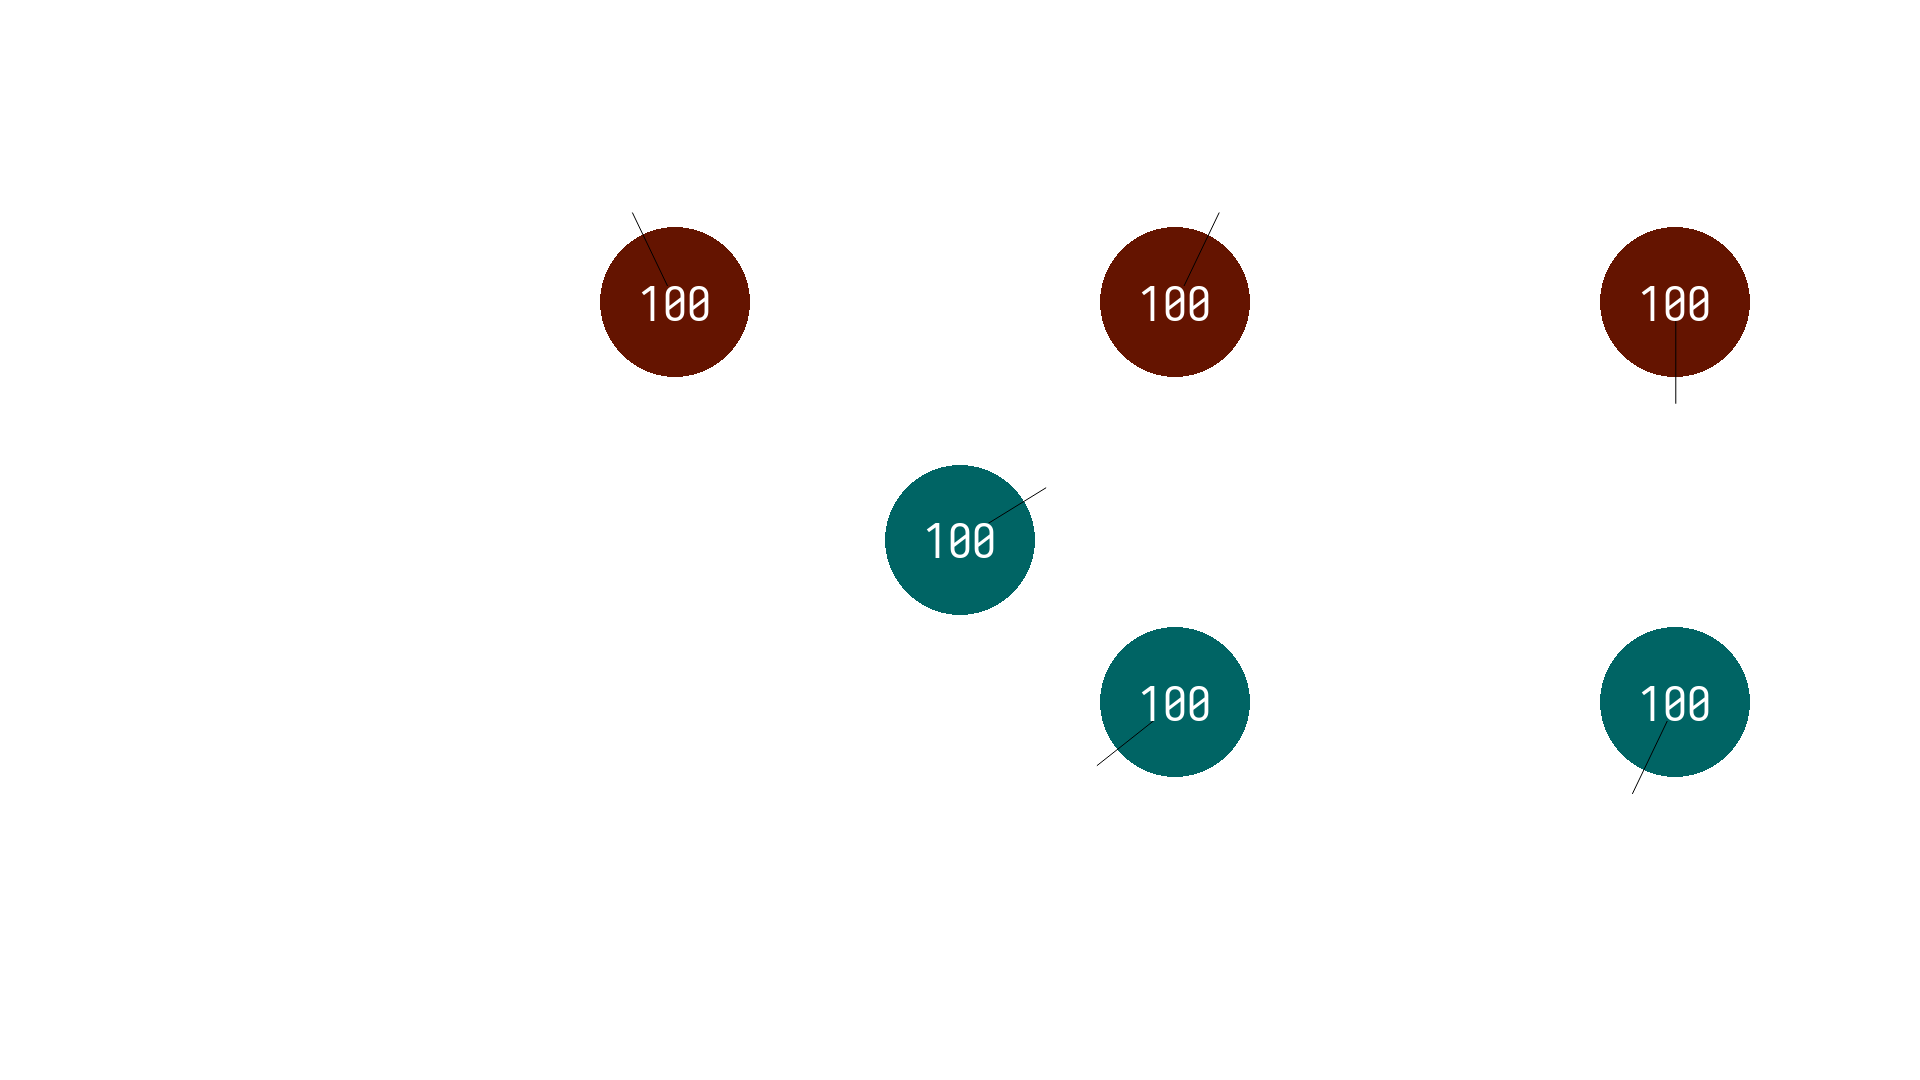
\includegraphics[width=\linewidth]{Development/Images/game_loop_4.png}}
    }
    \caption{A screen capture of the game loop with the health drawn on the players.}
    \label{fig:game_loop_4}
\end{figure}

We will now create \m{handleRayCollisions()} which takes in the \m{rays} dictionary containing all of the rays and which players were the source.

\begin{mpy}



\end{mpy}

\href{https://www.youtube.com/watch?v=VpSWuywFlC8}{Refer to this video since we will be doing collisions using rectangles not circle}

\href{https://gamedev.stackexchange.com/questions/199861/collision-detection-between-moving-objects-in-pygame}{This one might help too just take a look.}
